
It is not possible to cover in a single chapter all the technical development in radar instruments and their processing over the last 50 years. We will thus focus mostly on nadir radar altimeters with some discussion of complementary measurements from Synthetic Aperture Radar (SAR) and wave spectrometer systems. Hopefully more chapters will pop up in Part 3 to go beyond 
this presentation. 

\section{General considerations about radar remote sensing}
Since the invention of radar, the sea was found to be an important source of echoes, at all radar frequencies (from decametric to micro waves). 
This is due to the dielectric properties of sea water. An active radar measures the electromagnetic power received by its antenna. Using the radar equation, this power (in Watts)
is normalized by the antenna-target distance, the antenna size, and the emitted power. This gives the normalized radar cross section (NRCS), a quantity without dimensions that is often represented 
by the symbol $\sigma_0$. 
$\sigma_0$ depends on the surface geometry but it also varies with the radar frequency and polarization,  and observation direction (azimuth and incidence angles). %In particular, $\sigma_0$ highly depends on the radar wavelength and of the wave radar incidence angle relative to the surface.
The phase properties of the signal can also be used to estimate velocities at the ocean surface: current and wave orbital velocities \citep{Nouguier&al.2018,Rodriguez2018}. 

%A down-looking (nadir) radar will measure a high $\sigma_0$ for a smooth sea surface. If waves are present, the surface echoes may be considered as the incoherent superposition of the facet echoes. 
%%%%%%%%%%%%% figure
\begin{figure}[htb]
\centerline{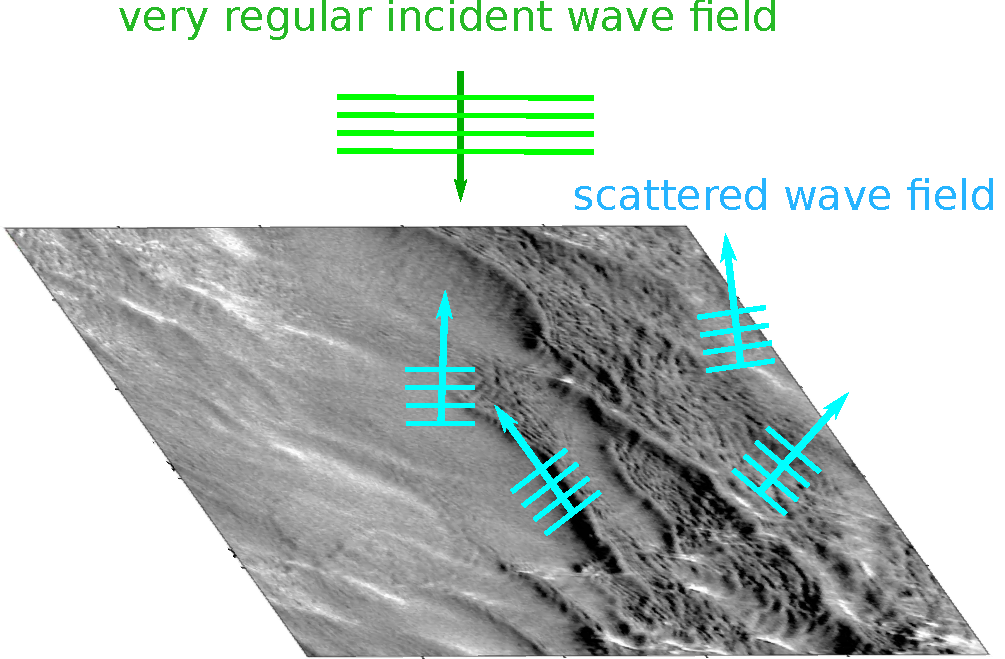
\includegraphics[width=0.5\textwidth]{FIGS_CH_SAT/scatter.pdf}}
%\vspace{3.64in}
  \caption{Conceptual schematic of microwave radar waves scattering at the sea surface. The grey shades are an example of a map of surface slopes estimated from a polarimetric system and covering a region of about 1 by 1 meter \citep{Laxague&al.2018}.  Note that the scattered (radar) wave field strongly varies with radar frequency, incidence and azimuth angles,  and polarization.  }\label{fig:scatter}
\end{figure}
%%%%%%%%%%%%% end of figure
Before we look at radar power or phase, one should have in mind a few important facts:
\begin{itemize}
\item within the radar field of view, the echoes recieved by the radar are coming from only a very small fraction of the surface. 1) Where the ocean is smooth (at the scale of the radar wavelength) only those pieces of the ocean surface that are facing the radar will contribute to the measured reflected signal. 2) Where the surface is curved, there will be a very weak scattering in all directions. 
\item the many echoes on the sea surface have randomly distributed distances (and velocities) relative to the radar, so that  the relative phases of all the echoes are randomly distributed and the sum of the electric fields of all these random echoes will have highly fluctuating amplitudes within a few milliseconds as the ocean surface moves: this effect is called "Rayleigh fading" and it introduces speckle noise in the radar measurements. This is very similar to the presence of wave groups in narrow-banded wave spectra. 
\end{itemize}

The radar wavelength 
and frequency are related by the speed of light $c$, namely $f_r = c / \lambda_r$. Different frequency bands have been reserved for Earth remote sensing, although they can be contaminated by military radars and other 
systems. Note that telecommunication systems (FM radio, TV channels, GSM networks, GPS/Galileo positionning systems ...) use different bands in the microwave range, and remote sensing may use these sources of opportunity for signals that reflect off the sea surface  \citep[e.g.][]{Lowe&al.2002}.
%%%%%%%%%%%%%%%%%%%%%%%%%%%%%%%%%%%%%%%%%%%%%%%%%%%%%%%%%%%%%%%%%%%%%%%%%%%%
\begin{table}[hb]
  \centering
  \begin{tabular}{|c|c|c|c| c |}
 \hline
band name & frequency & wavelenghth & example instrument & satellite  carrying the instrument  \\
 \hline
W  & 94 GHz  & 0.3 cm & CPR & Cloudsat  \\
Ka & 30 GHz  & 0.8 cm & AltiKa or KaRIN & SARAL or SWOT  \\
Ku & 15 GHz  & 2.2 cm & Poseidon 3 & Jason 3  \\
X &  9.6 GHz & 3.1 cm & & TerraSAR-X  \\
C & 6 GHz   & 5 cm & Poseidon 3 or ASCAT & Jason 3 or MetOp \\
S & 3 GHz   & 12 cm & S-SAR &  NISAR \\
L & 1.5 GHz  & 24 cm & SMAP  & SMAP \\
P & 435 MHz  & 70 cm & P-SAR & Biomass (launch  in 2024 or 2025) \\
\hline
\end{tabular}
\caption{Typical average frequencies and wavelengths used for ocean remote sensing in the different radar microwave bands. The actual frequency usually varies during a radar pulse with a bandwidth $B$ that defines 
the range resolution of the instrument. \label{table_radars}}
\label{table_bands}
\end{table}
%%%%%%%%%%%%%%%%%%%%%%%%%%%%%%%%%%%%%%%%%%%%%%%%%%%%%%%%%%%%%%%%%%%%%%%%%%%%
Ocean waves have been monitored from space continuously since the lauch of ERS-1 using altimeters (looking straight down)  and SARs (generally looking to the side), as summarized in figure \ref{fig:satellite}: note that with the exception of CFOSAT, no satellite was ever designed for measuring waves. Waves are a by-product, sometimes necessary for other measurements. Altimeters generally combine different radar frequencies to be able to correct for specific time delays in the propagation through the ionosphere, while additional radiometers provide correction for tropospheric time delays.  Some satellite missions also include both SARs and altimeters. In the case of SWOT the pair of SARs constitutes the across-track interferometer KaRIN which also measures the elevation of the sea surface at very high resolution, but across a narrower (120 km) swath that other SARs. Any satellite may carry many different instruments, and it is often easier to use the instrument name to avoid any confusion: SWOT carries both a Poseidon-3 altimeter (like Jason 3) and KaRIN. 

%%%%%%%%%%%%% figure
\begin{figure}[htb]
\centerline{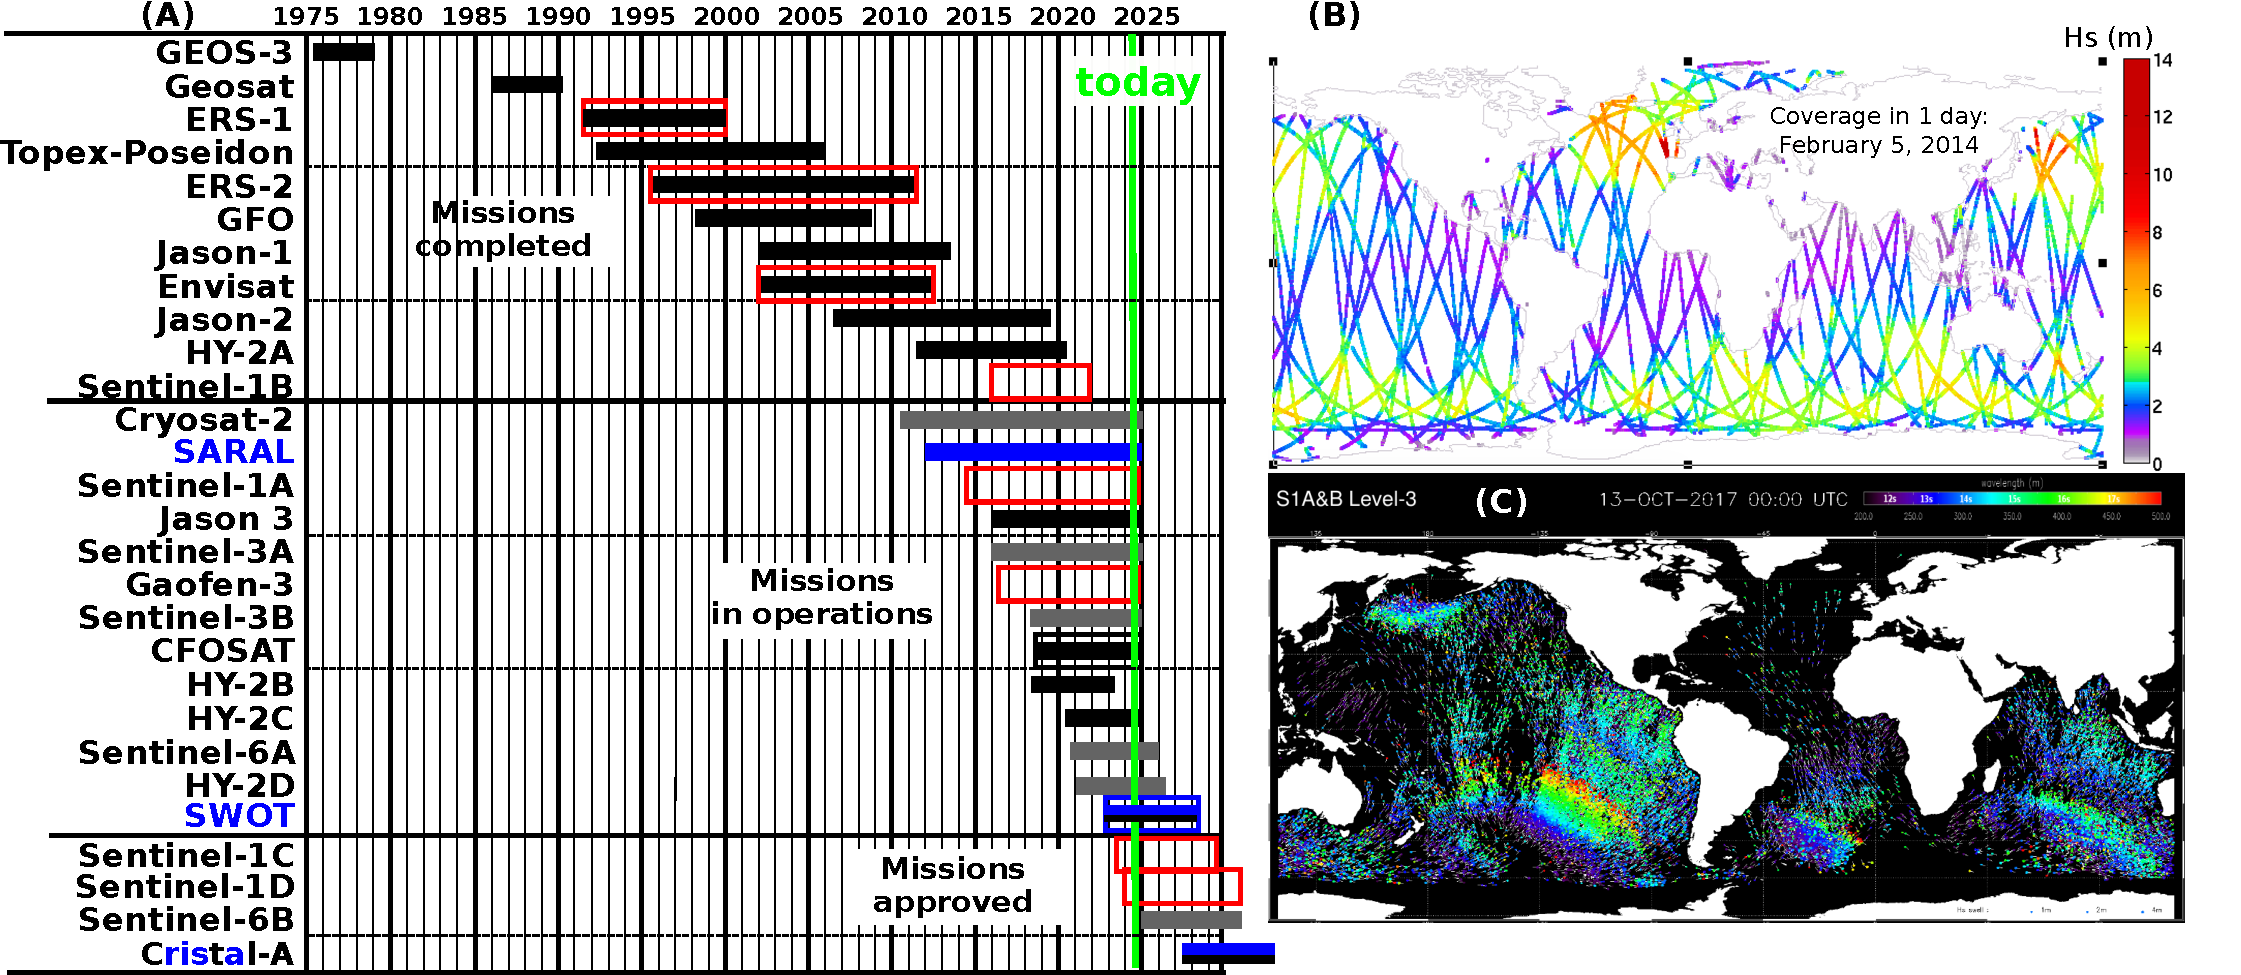
\includegraphics[width=\textwidth]{FIGS_CH_SAT/missions.pdf}}
%\vspace{3.64in}
  \caption{Satellite missions with sea state monitoring objectives.}
    {Time coverage of satellite missions from 1985 to 2030, including nadir and near-nadir altimeters (solid bars), and missions monitoring ocean wave spectra (open boxes) using C-band Synthetic Aperture Radars (red), and real aperture radars in Ku-band (black) or Ka-band (blue). The lighter color (grey and blue) bars correspond to altimeters using Delay-Doppler processing. Source: CEOS database
    \url{http://database.eohandbook.com/}). (B) example of 1-day coverage for Hs measurements with 4 satellite altimeters 
    (C) snapshot of a 'fireworks' plot, the showing the height (size of symbols) peak periods (colors), and directions (barbs) of 
    swell partitions derived from Sentinel-1A and Sentinel-1B wave mode data. Such plots are produced routinely by CMEMS.}\label{fig:satellite}
\end{figure}
%%%%%%%%%%%%% end of figure



For any application (measuring sea level, wind speed, ... ) the choice of the radar frequency is dictated by 
a number of considerations, including atmospheric absorption, as we want to be able to measure a returning echo from the sea surface, and the 
size of the antenna. In particular, low frequencies give large wavelength that require a proportionally large antenna to have a narrow beam. A very narrow beam (tens of meters) is only achievable with visible light (lidars). Radars will typically collect echoes from a region that is several kilometers across, which is good as we generally wish to average over the waves to measure non-wave properties (such as sea level). A wide beam makes it possible to cover a wide area, which is nice if we can "slice" the data into smaller "radar pixels". The most simple way to slice the data is transmit "chirps", radar pulses with a carrier frequency that sweeps a bandwidth $B$. The standard \href{https://en.wikipedia.org/wiki/Pulse_compression}{pulse compression technique} is able to separate\footnote{The separation is not perfect and there is always some "mixture" of signals from neighboring pixels (in radar jargon, the Point Target Response, or PTR, is not a delta function).} echoes as a function of their distance from the radar, with a resolution that is $\delta_R=c/2B$.  This is another reason for using higher frequencies: most radar altimeters have used Ku band and a bandwidth $B=320$~MHz which gives a resolution $\delta_R=47$~cm. It is easier to fit a wider bandwidth at higher frequencies, as was done with AltiKa on SARAL, using $B=500~MHz$ that gives $\delta_R=30$~cm. So how can we measure sea level within a few centimeters given these rather large resolution?  Well, we don't measure sea level: we estimate it from the actual measurement which is the radar waveform. These resolutions also explain why nadir altimeters can't distinguish very well between 10 cm and 40 cm wave heights.


\section{Altimeters waveforms and the Brown-Hayes model}
%Radar altimeter data are, the source of measurements of $H_s$  available at global scale and used for operational wave forecasting
%through data assimilation. Contrary to other observation systems, $H_s$ is directly estimated, without the use of a spectral analysis. The usual 
%arrangement is a radar antenna looking straight down - at the nadir - on the the sea surface. 

%%%%%%%%%%%%% figure
\begin{figure}[htb]
\centerline{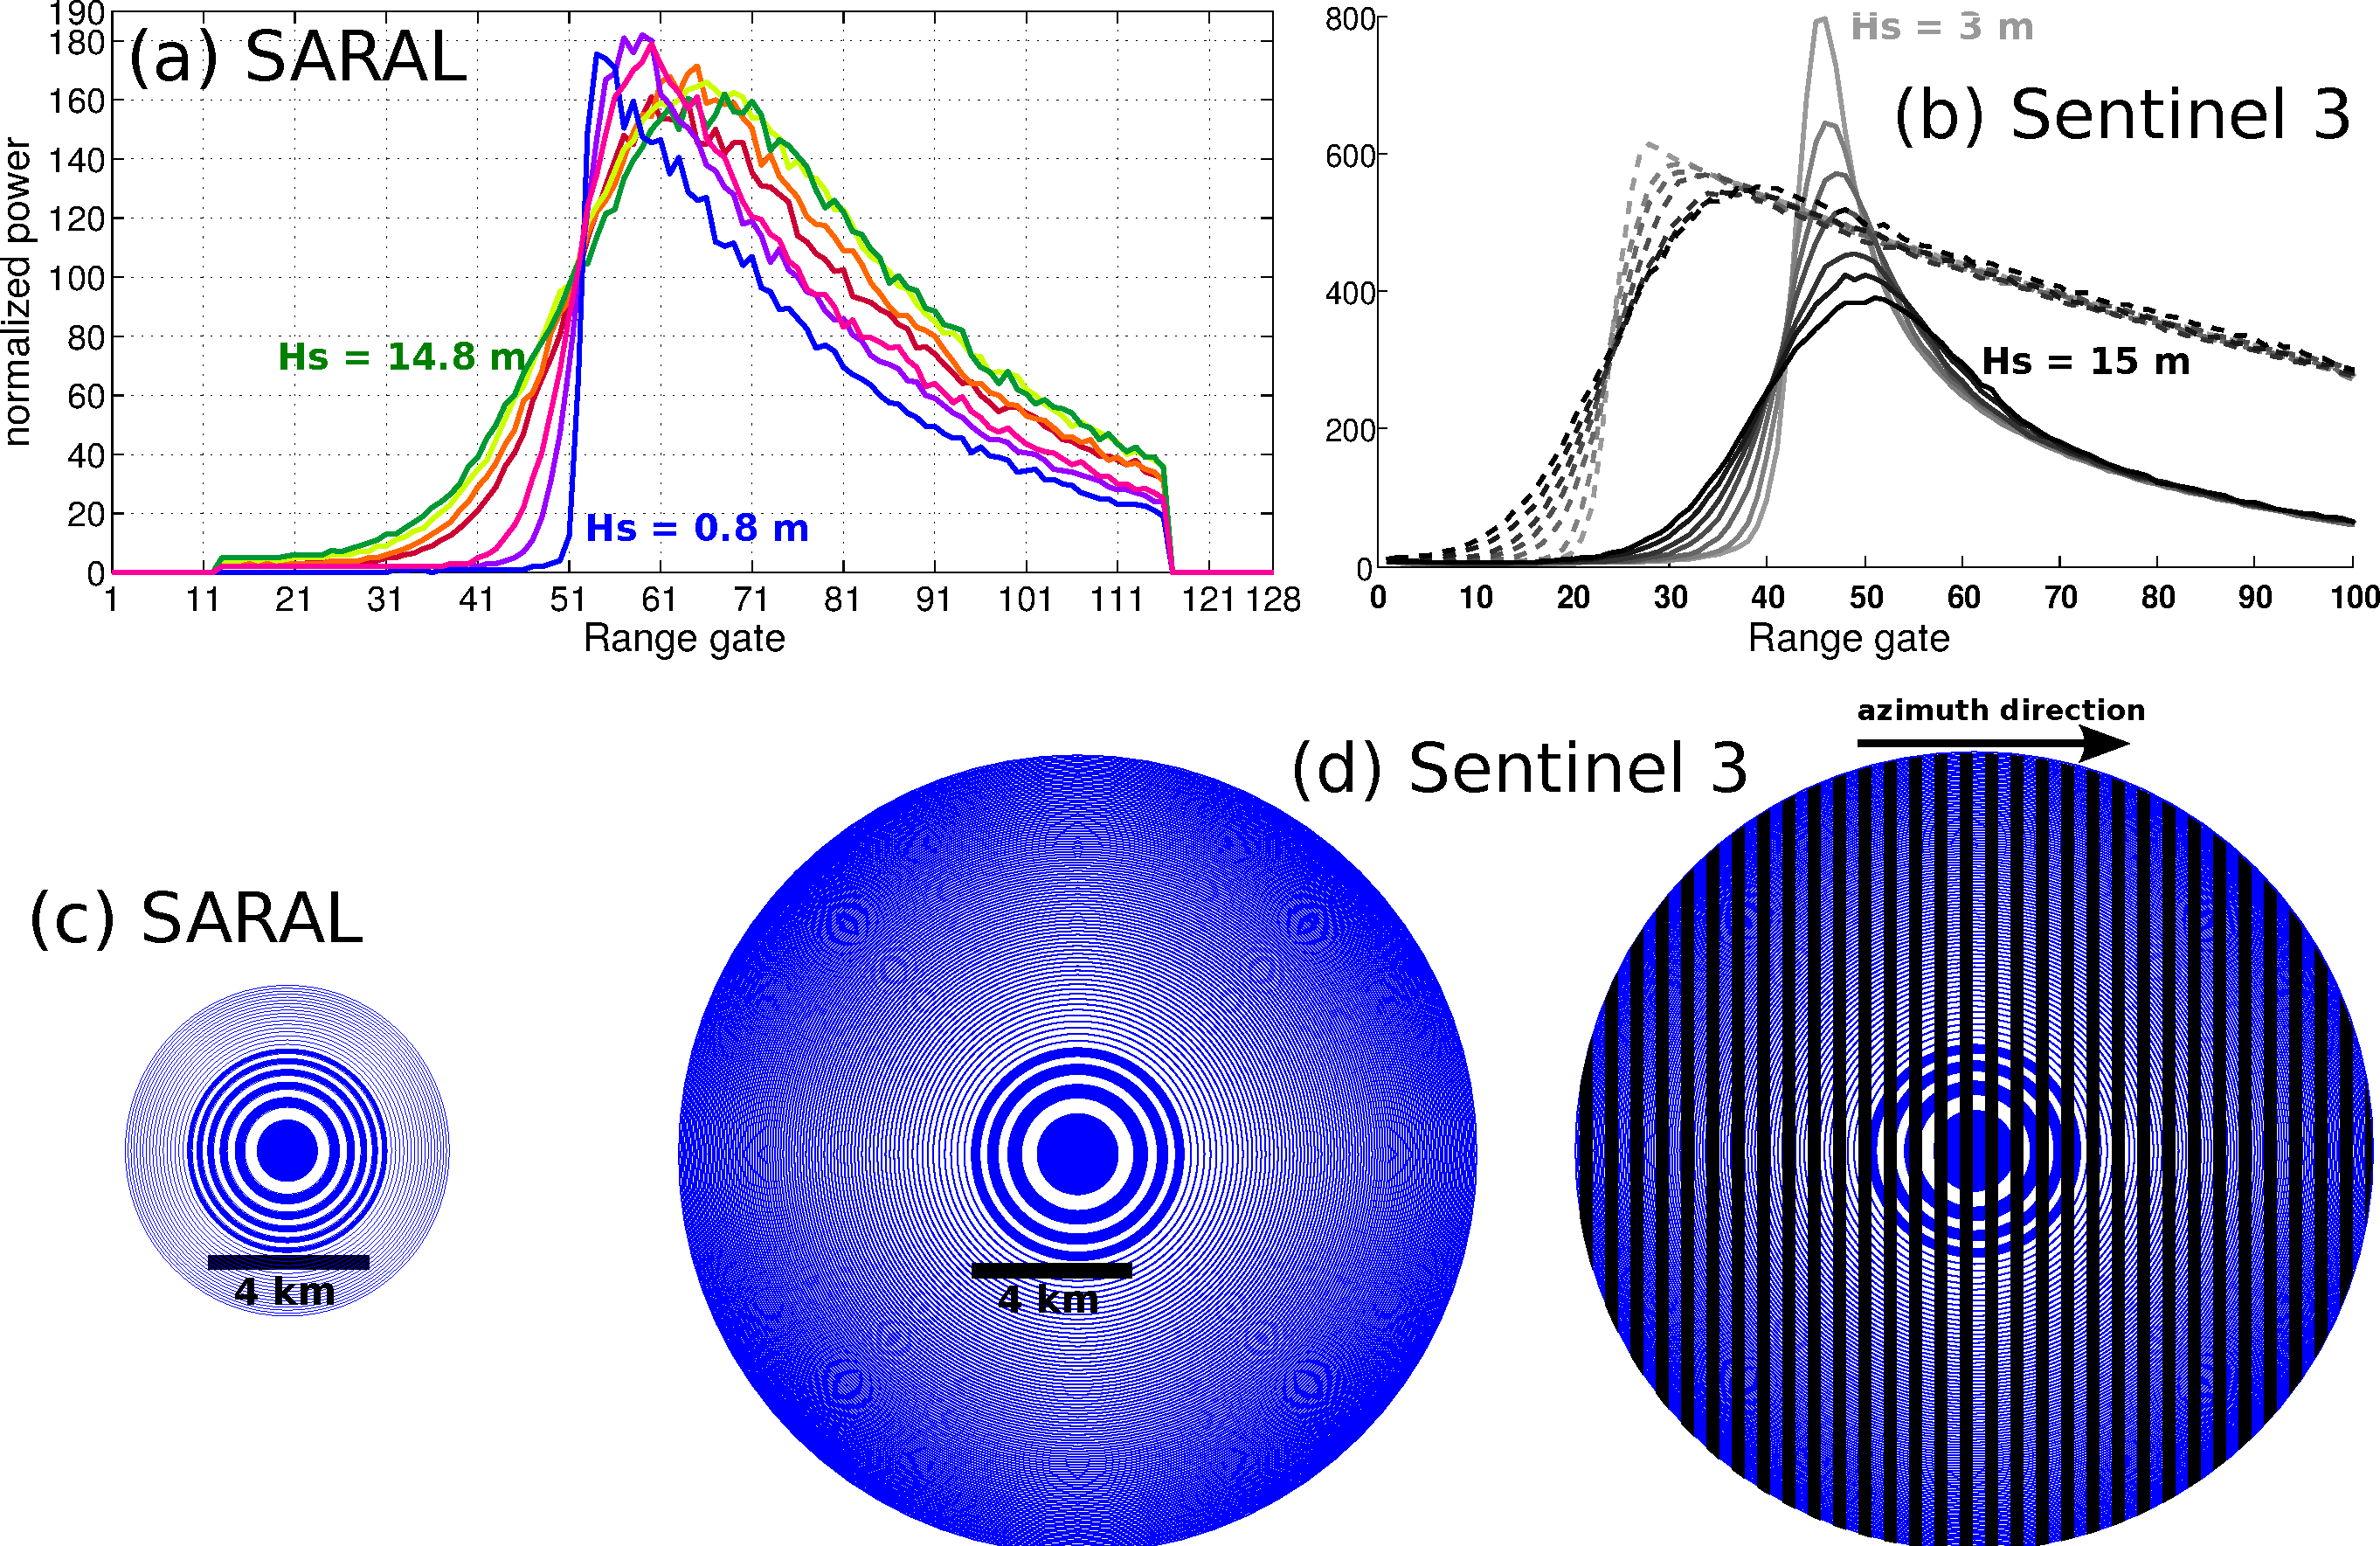
\includegraphics[width=0.9\textwidth]{FIGS_CH_SAT/dessin_footprint.pdf}}
%\vspace{3.64in}
  \caption{Altimeter waveforms and footprints}
    {Example of altimeter waveforms for different wave heights.}
    {(a) These waveforms were selected along the ascending track of SARAL/AltiKa on February 5, 2014, 
    beteen 05:29:49 and 06:20:07 UTC. Each waveform shows the the power measured by the radar as a function of time: 
    time is discretized with intervals of $2 \times 10^{-9}$~s corresponding to 
30~cm range intervals usually called `range gates'. The corresponding wave heights are 0.8, 3.2, 4.6, 9.7, 10.7, 13.2, and 14.8 m. 
Data is available from CNES/Aviso ftp. Each waveform shown here was obtained for 1~s of data, 
 as the median of 40 conscutive waveforms. (b) Similar waveforms from Sentinel 3 using delay-only (dashed) and delay-doppler (solid) for Hs = 3,5,7,9,11,13
and 15 m, for cycle 23 orbit 349, on 25 October 2017 in the Pacific. (c) Spatial coverage of footprints corresponding to the 3-dB antenna lobe pattern, for an 
unrealistic flat sea surface with a uniform roughness, with the first 11 range gates painted alternatively blue and white, 
starting from center. (d) Footprint for Sentinel 3, with the 7 seven range gates colored blue and white, with the azimuth resolution of the Doppler processing indicated by the grey stripes.
} \label{waveform}
\end{figure}
%%%%%%%%%%%%% end of figure
The first main principle of the analysis of the radar echoes is the determination  of the distance, usually called range, based on 
the delay of a radar pulse to travel from the transmitting antenna to the target and back to the receiving antenna. Usually the two antennas are the same piece of hardware 
and this is called a `monostatic system'. Because the radar pulse has a finite duration which limits the resolution of the time measurement, 
it is customary to use a varying transmitted carrier frequency $f_t$ that is modulated as chirps: $f_t$ is increased linearly between $f_0$ and $f_0$+$B$ during a radar pulse. As a result, the carrier frequency of the received signal $f_r$ can be used to determine the precise travel time of the received pulse, with each frequency associated to a different range $r$, with a resolution in range $dr$ that is determined by the frequency bandwidth $B$, with $dr=c /(2B)$. The actual signal at frequency $f_r$ combines echos from all ranges convoluted by the point target response \citep[e.g.][]{Halimi2013}.  

%for all types of radars, it is thus better to use a larger bandwidth, 
%but this is usually limited by atmospheric absorption windows or telecommunication regulations. Hence, for satellite altimeters, $B$ for the Jason altimeters is 320~MHz  
%giving $dr=48$~cm. SARAL/Altika used a wider bandwidth of  
%500~MHz  giving $dr=30$~cm. Because of issues with rain attenuation, all altimeters since GEOS-3 (1975-1979) have used Ku-band, except for the ongoing SARAL/AltiKa mission which uses only Ka-band.

Each radar pulse emitted by the radar antenna is  reflected by an ocean area that expands with time, starting from the blue disk in the middle of figure \ref{waveform}.c, and 
expanding to the outer rings. The shape of the blue disk is only correct for a flat sea surface, and is distorted by waves as the crests give a shorter range and the troughs give a higher range. 
the radar receives echoes from wave crests firsts and wave troughs later: this difference in travel time between crests and troughs  
spreads the echoes over time. \cite{Brown1977} showed how the shape of the `waveform',  i.e. the received power return, under a number 
of simplfiying assumptions, is a convolution 
of the radar antenna pattern and the distribution of the surface elevation $\zeta$: if we assume that the surface elevation for each 
distance (range) follows a Gaussian distribution of standard deviation $\sigma_H=H_s/4$, a uniform distribution of specular points, and in the most simple case of a "flat surface response" in which the echo is 0 for ranges less than the satellite altitude $h_{\mathrm{o}}$ and 1 otherwise, then the Brown waveform is a sum of many shifted Gaussians. If we only had echoes from the region straight down below the satellite (this is called the nadir), the waveform would be a Gaussian. As we add a Gaussian for each region of the ocean located at a radius $r$ from the nadir, the echoes are Gaussian distributed but arrive a little later, with a time difference $2 \sqrt{(r+h_0)^2-h_0^2}/c$, and the waveform is the sum of all these shifted Gaussians.  This sum is a particular function that is called the error function, erf, and the  theoretical waveform as a function of time is, 
\begin{equation}
    w_B(t,t_0,\sigma_t,\sigma_0)=  \sigma_0 \left\{ 1+ \mathrm{erf}\left[(t-t_0)/( \sqrt{2} \sigma_t) \right] \right\}, \label{Brown}
\end{equation}
with $\sigma_s$ the standard deviation of the travel time from the scatterers to the radar, with is converted from their spatial distribution with $\sigma_t= 2 \sigma_H / c$, with $c$ the speed of light. Likewise the mean radar pulse travel time $t_0$ is related to the mean sea level relative to the satellite is $t_0=2(h_o- z_e)/c$. The last parameter $ \sigma_0$ is the Normalized Radar Cross section which depends on the "surface roughness" and will be further discussed below. We thus have a waveform that is a function of three geophysical quantities that depend on the surface geometry: a mean sea level, a standard deviation of the sea level (a.k.a. $H_s/4$) and roughness parameter. This shape is a good approximation of the "leading edge" of the true waveforms (the rising part of the curves in figure \ref{waveform}. The fact that the true waveform also have a decreasing part is due to the finite aperture of the 
radar beam, which gives a multiplicative term $\exp(-c_\xi (t-t_0)+c_\xi^2 \sigma_t^2/2)$ that was neglected in eq. (\ref{Brown}).  %adds a exponential decay term, 
%\begin{equation}
%    w_B(t)=  \sigma_0 \left\{ 1+ \mathrm{erf}\left[(t-t_0)/( \sqrt{2} \sigma_t) \right] \right\}, \label{Brown_ant}
%\end{equation}


As a result, 
the slope of the `wave form leading edge' is proportional to  $H_s$.  
In the case of the largest sea state in figure \ref{waveform}.a, the return 
power spreads over about 35 range gates, from number 26 to number 61, i.e. a distance of 10.5~m, close to the root mean square wave height
 $H_{\mathrm{rms}} \approx  H_{s}/1.4$. %The power in range gates beyond 50 comes from the sea surface that is not directly 
% under the satellite but on a circle around it, and is still illuminated by the radar beam.  

\subsection{The mean square slope (mss)}
The backscattered power $\sigma_0$ is nearly inversely proportional to the mss \citep{Vandemark&al.2002}. 
For display purposes the waveforms shown in figure \ref{waveform} have been scaled: you can see that the noise level (power in gates 11 to 21) which should be nearly the same for 
all sea states is scaled to lower values for lower sea states that generally have low values of both $H_s$ and mss.  
Because the mss is not a very common parameter in applications, many authors have derived empirical estimates of peak or mean  periods from $H_s$ and $\sigma_0$. Also, the mss is a good proxy for the wind speed \citep{Cox&Munk1954}.




\subsection{The effective footprint of nadir altimeters}
The backscattered power $\sigma_0$ is nearly inversely proportional to the mss \citep{Vandemark&al.2002}. 
For display purposes the waveforms shown in figure \ref{waveform} have been scaled: you can see that the noise level (power in gates 11 to 21) which should be nearly the same for 
all sea states is scaled to lower values for lower sea states that generally have low values of both $H_s$ and mss.  
Because the mss is not a very common parameter in applications, many authors have derived empirical estimates of peak or mean  periods from $H_s$ and $\sigma_0$. Also, the mss is a good proxy for the wind speed \citep{Cox&Munk1954}.



But what region of the ocean does this correspond to? \cite{Chelton&al.1989} made a first estimate of the size of the "oceanographic footprint": he reasoned that one can neglect the probability that the sea level may be at $\zeta > H_s$ above the local mean sea level (you can check on $p(\zeta > H_s)$ assuming a Gaussian distrubution)  so that at $t=t_0$ there are no echoes coming from a distance $\rho > \rho_C$ from the nadir.  Using the Pythagorean theorem (assuming the Earth is flat), this neglects the unlikely echoes would contribute to the waveform at $t=t_0$ if their range is $h_o=\sqrt{(h_o-H_s)^2-\rho_C^2}$.  Equivalently this neglects the contribution of nadir echoes at $z< -H_s$ that could mix with echoes from $(z=0,\rho=\rho_C)$ as shown in Figure \ref{fig:group_alti}.
%%%%%%%%%%%%% figure
\begin{figure}[htb]
\centerline{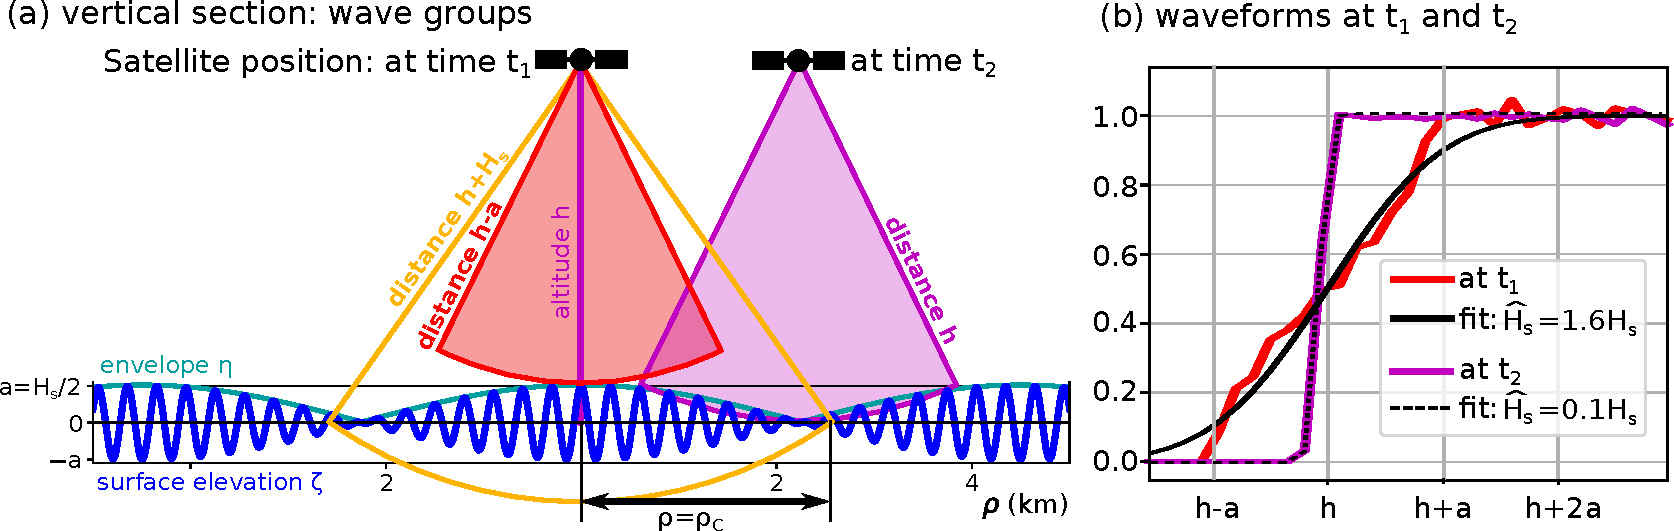
\includegraphics[width=\textwidth]{FIGS_CH_SAT/wave_group_schematic.pdf}}
%\vspace{3.64in}
  \caption{Schematic of altimeter measurements in the presence of long wave groups and definition of the \cite{Chelton&al.1989} radius $\rho_C$.}{} \label{fig:group_alti}
\end{figure}
%%%%%%%%%%%%% end of figure
\begin{equation}
    \rho_C =\sqrt{h_o^2- (h_o-H_s)^2} \simeq \sqrt{ 2 h_o H_s} \label{eq:rC} 
\end{equation}
For a more realistic spherical Earth, there is a $1/(1+h_o/R_E)$ correction factor inside the square root, with $R_E$ is the Earth radius, given by simple geometry considerations  \citep{Chelton&al.1989}.

This estimate of the radius of the "oceanographic footprint" is very conservative. In practice it is not important if the parameters to be estimated are uniform at scales greater than $\rho_C$. But as are trying to squeeze out more and more information from satellite measurements, can we be more precise in the spatial resolution of these measurements?  On Figure \ref{fig:group_alti}.b, the fitting of the simulated waveforms ranges from 0.1 $H_s$ to 1.6 $H_s$: an altimeter measures a local wave height that can only gives the significant wave height when averaged over the wave groups. If we assume the local wave height is a properly scaled average of the envelope of the wave groups (you can check that $H_l=4\sqrt{2/\pi} \eta$ gives the proper average), then 0.1  $H_s$  is an average over about 0.25 $\rho_C$. How can we define this exact number? Is it also true for shorter wave groups? 



%Classical altimeter estimates of $H_s$ are fairly noisy when the wave height is low becase in that case $H_s$ is determined by only very few range gates, and the power in each rage gate as a random noise, also called speckle noise, caused by Rayleigh fading of ocean echoes that are coming from ranges spread over a distance much greater than the electromagnetic wavelength hence with random phases that randomy cancel \citep{Quartly&al.2001}. 
%\cite{DeCarlo&al.2023} showed that wave groups introduce fluctuations in the estimated values $\widehat{H}_s$ that are proportional to $H_s$ and the spectral peakedness parameter $Q_{kk}$, introduced in chapter \ref{ch_groups}, these fluctuations can be dominant for the largest wave heights. 




\section{Fitting the waveforms}

The practical method for estimating the three parameters, is to find the values for the sea level $\widehat{z}_e$, wave height $\widehat{H}_s=4 \widehat{\sigma}_H= 2 c \widehat{\sigma}_t$, and $\widehat{\sigma}_0$ that minimize a cost function. The most simple case is to use a the least square cost 
function. With a measured waveform $(w_k)$ discretized with a resolution $\delta_t$, we search for the values  $\widehat{t}_0$, $\widehat{\sigma}_t$, $\widehat{\sigma}_0$ that minimize 
\begin{equation} 
    C_{\mathrm{LS}}(t_0',\sigma_t',\sigma_0')=\sum_{k=k_{\min}}^{k_{\max}}  \left[ w_k - w_B(k \delta_t,t_0',\sigma_t',\sigma_0') \right]^2. \label{eq_CLS}
\end{equation}
For a perfect ocean and perfect instrument we have a measured waveform that follows eq. (\ref{Brown}) and the cost function is zero (and minimum) for 
$\widehat{t}_0=t_0$, $\widehat{\sigma}_t=\sigma_t$, $\widehat{\sigma}_0=\sigma_0$. For the real ocean, we get something that is a little different. 

An interesting case is the effect of spatial variations in the local wave height. In the most simple case we imagine a local wave group with a wave height $H_s(1+\Delta)$. We will assume that this perturbed wave height is present in an area $A_0$ that is small compared to what we define as the equivalent footprint area $A_e= \pi \rho_C^2/4$, and centered around the radius $\rho_0$ corresponding to the travel time $t_\rho$. For $A_0/A_e \ll 1$, the waveform is obtained by replacing the local Gaussian distribution $G$ in the area $A_0$ by a different Gaussian distribution, giving the analytical expression 
\begin{equation}
    w(t,t_0,\sigma_t,\sigma_0,\Delta, A_0,\rho_0)=  w_B(t,t_0,\sigma_t,\sigma_0) + w'(t,t_0,\sigma_t,\sigma_0,\Delta, A_0,\rho_0)
\end{equation}
with the perturbation 
\begin{equation}
    w'(t,t_0,\sigma_t,\sigma_0,\Delta, A_0,\rho_0) = \sigma_0 \frac{A_0 }{ \pi c h_o} \left[ G((1+\Delta)\sigma_t,t_0,t-t_\rho)- G(\sigma_t,t_0,t-t_\rho)  \right].
\end{equation}
where the normalization factor $\pi c h_o$ is the area of a ring of unit width $2 \pi \rho_0$ multiplied by $c h_o / 2 \rho_0$ to convert the unit width to unit travel time. If that sounds strange, it is because I'm trying to avoid stepping back to the elevation PDF and adding 2 more equations to compute the waveform as a convolution of that PDF, as done  in Appendix A of \cite{DeCarlo&Ardhuin2024}.  
%%%%%%%%%%%%% figure
\begin{figure}[h!]
\centerline{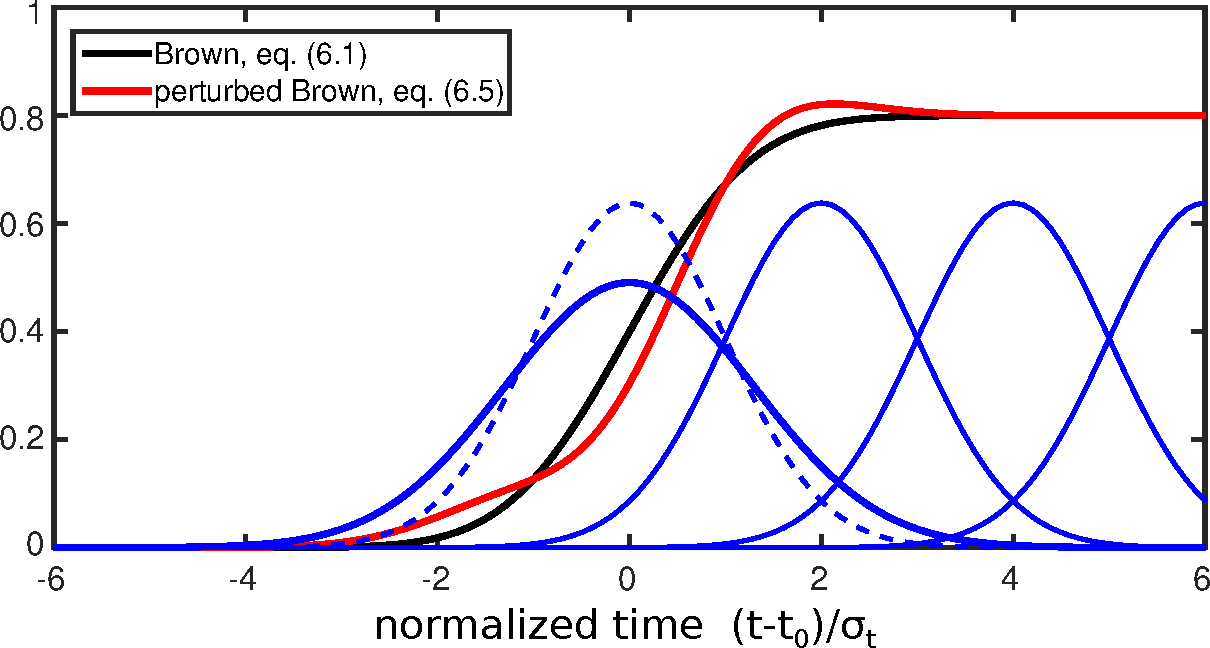
\includegraphics[width=0.8\textwidth]{FIGS_CH_SAT/waveforms_perturbation.pdf}}
%\vspace{3.64in}
  \caption{The waveform is the sum of the PDF of surface elevation(in blue) shifted by their Waveform perturbation caused by a localized wave group at nadir ($b=0$) with a perturbation amplitude $a=\Delta A_0/A_e=0.3$}{} \label{fig:group_alti_perturb}
\end{figure}
%%%%%%%%%%%%% end of figure

We can now use a Taylor expansion to replace the difference by $\Delta$ times the derivative of $G$ with respect to $\sigma_t$, which gives, 
\begin{equation}
   w'(t,t_0,\sigma_t,\sigma_0,\Delta, A_0,\rho_0) \simeq   \sigma_0 a p(t- 4 b \sigma_t,t_0,\sigma_t)
\end{equation} 
with 
\begin{eqnarray}
        a&=&\Delta \frac{A_0}{A_{\mathrm{e}}}  =\Delta \frac{2 A_0}{\pi h H_s} \label{eq:alti_a} \\ 
    p(t,t_0,\sigma_t) &=& \frac{1}{\sqrt{2\pi}} \mathrm{e}^{-0.5 \left(\frac{t-t_0}{\sigma_t} \right)^2 } \left[\left(\frac{t-t_0}{\sigma_t} \right)^2-1\right]. \label{eq:p_alti} \\
        b&=& \left(\rho_0/\rho_C \right)^2
\end{eqnarray} 


This non-Brown waveform can be retracked analytically, in particular by approximating the discrete sum in the cost function with a continuous integral, we get an analytical expression for the cost function. Using the notation $w_B'=w_B(t,t_0',\sigma_t',\sigma_0')$, we have, 
\begin{eqnarray}
   C_{\mathrm{LS}}(t_0',\sigma_t',\sigma_0')& \simeq &\int_{-\infty} ^\infty \left( w-w_B'  \right)^2 \mathrm{d} t =\int_{-\infty} ^\infty \left( w_B+w'-w_B'  \right)^2 \mathrm{d} t \\
                  & \simeq & \int_{-\infty} ^\infty \left( w_B-w_B' \right)^2  + w'^2+ 2 w'\left( w_B-w_B' \right)  \mathrm{d} t 
\end{eqnarray} 
It is relatively simple to find the minimum of this function \citep{DeCarlo&al.2023} by Taylor expanding $w_B-w_B'$, 
\begin{equation}
    w_B-w_B' \simeq  (t_0-t_0') \frac{\partial w_B}{\partial t_0} +   (\sigma_t-\sigma_t') \frac{\partial w_B}{\partial \sigma_t} +   (\sigma_0-\sigma_0') \frac{\partial w_B}{\partial \sigma_0} + (t_0-t_0')(\sigma_t-\sigma_t') \frac{\partial^2 w_B}{\partial t_0  \partial \sigma_t}  \dots 
\end{equation}
Plugging this into the cost function gives a second order polynomial 
\begin{eqnarray}
   C_{\mathrm{LS}}(t_0',\sigma_t',\sigma_0')& \simeq & (t_0-t_0')^2 \int_{-\infty} ^\infty \left(\frac{\partial w_B}{\partial t_0}\right)^2 \mathrm{d} t + (t_0-t_0') \int_{-\infty} ^\infty w' \frac{\partial w_B}{\partial t_0} \mathrm{d} t   +  \dots \\
     & \simeq & (t_0-t_0')^2  I_{t_0,2} + (t_0-t_0') I_{t_0,1} +  (\sigma_t-\sigma_t')^2  I_{\sigma_t,2}  +  (\sigma_t-\sigma_t')  I_{\sigma_t,1} + \dots
\end{eqnarray} 
where all the integrals $I_{x,2}$ are independent of the perturbation $w'$ and   $I_{x,1}$ are analytical functions of the $w'$ perturbation parameters, here $a$ and $b$. The cost function is thus minimum where the derivatives are zero. If we neglect the second order cross derivates we get
\begin{eqnarray}
\partial C_{\mathrm{LS}} / \partial (t_0-t_0') &= & 2 (t_0-t_0')    I_{t_0,2} + I_{t_0,1}  \\
\partial C_{\mathrm{LS}} / \partial (\sigma_t-\sigma_t') &=&  2 (\sigma_t-\sigma_t')    I_{\sigma_t,2} + I_{\sigma_t,1}    \\
\partial C_{\mathrm{LS}} / \partial (\sigma_0-\sigma_0') &= & 2 (\sigma_0-\sigma_0')    I_{\sigma_0,2} + I_{\sigma_0,1}   
\end{eqnarray} 
Because the integrals $I$ are simple linear expressions as a function of $w'$, the effect of perturbations $w'$ is linear and thus the effects od the different perturbations can be summed.  Also the cost function can be interpreted as a scalar product that is projecting the perturbation $w'$ on the gradients of the waveform function $w_B$. 

For our localized wave group we get the "analytically retracked" values, 
 \begin{eqnarray}
    \widehat{H}_{s}&=& H_s +  \frac{a H_s }{2}  J_H(b), \label{eq:Hsfit}\\
    \widehat{z}_e= - c \widehat{t_0} / 2 & =& - \frac{a H_s}{16} J_z(b),\label{eq:epochfit}
\end{eqnarray}
with 
%%%%%%%%%%%%% figure
\begin{figure}[h!]
\centerline{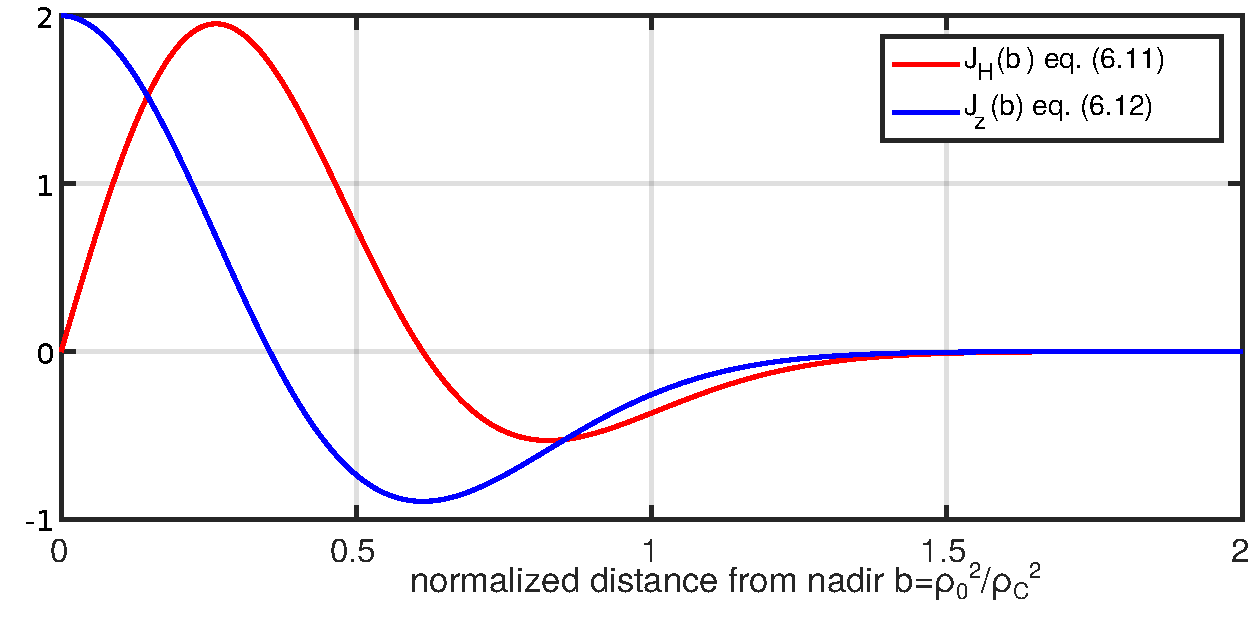
\includegraphics[width=0.8\textwidth]{FIGS_CH_SAT/FigA3_Jfunc.pdf}}
%\vspace{3.64in}
  \caption{Normalized perturbation of retracked wave height and sea level caused by a localized wave group at a distance $\sqrt{b} \rho_C$ from nadir. These functions are only valid for the simple least square cost function.}{} \label{fig:alti_JLS}
\end{figure}
%%%%%%%%%%%%% end of figure 
 \begin{eqnarray}
    J_H(b)&=& 2 b \left(6- 16 b^2\right) \mathrm{e}^{-4b^2},\label{eq:JH}\\
    J_z(b)&=&   \left(2-16 b^2\right) \mathrm{e}^{-4 b^2}.\label{eq:Jz}
\end{eqnarray}

This result is relatively surprising: a wave group localized at nadir (as in Figure \ref{fig:group_alti_perturb}) has no impact on the estimate of wave height, but it causes an error on the sea level estimate. This is responsible for most of the "hump", the spurious  along-track variability of sea level estimates. For wave heights the highest sensitivity is at $\rho=\rho_C/2$. When mapped over the ocean surface, the sensitivity kernel $J_H$ of the altimeter retracked with the LS cost function has a "doughnut" shape, as illustrated in Figure \ref{fig:alti_doughnut}. This theory allows to compute the value expected from altimeter retracking directly from a map of surface elevation, without the need to simulate the waveform and retrack it. 
%%%%%%%%%%%%% figure
\begin{figure}[h!]
\centerline{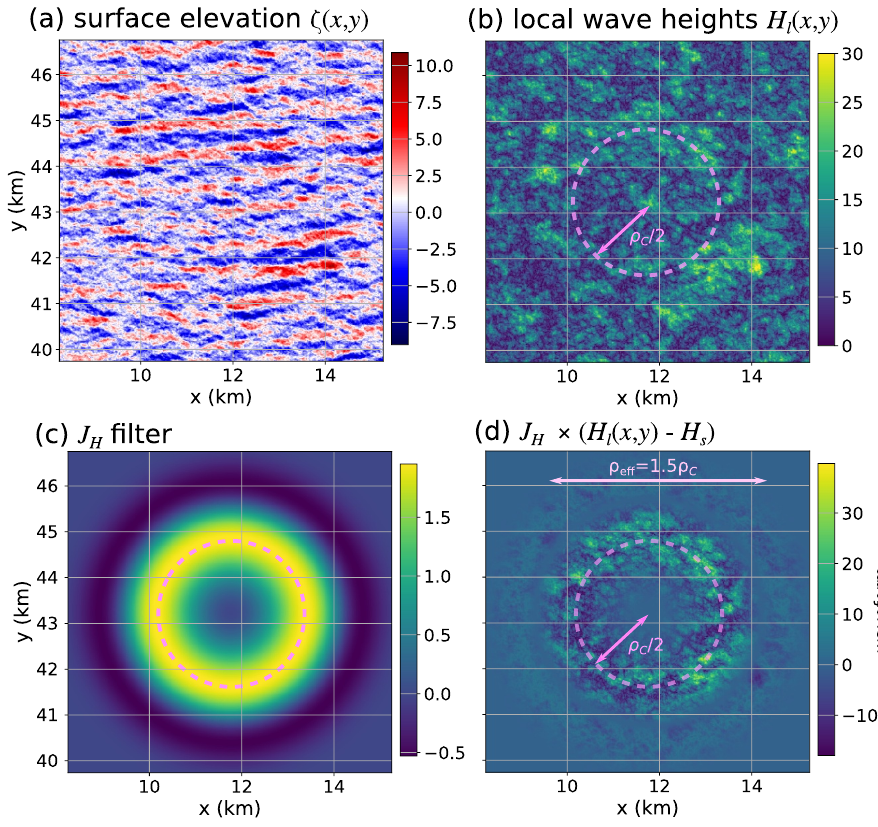
\includegraphics[width=0.7\textwidth]{FIGS_CH_SAT/doughnut-footprint-for-altimeters.png}}
%\vspace{3.64in}
  \caption{This figure shows simulated ocean surface elevation and local wave height, and the sensitivity of usual altimeter processing to the map of wave heights. The retracking of altimeter data is equivalent to smoothing the local vave heights with the filter $J_H$.}{} \label{fig:alti_doughnut}
\end{figure}
%%%%%%%%%%%%% end of figure 
This "doughnut theory" works in the sense that it predicts most of the variability in speckle-free simulations of altimeter waveforms. It does not predict all the variance because the phase of the waves introduce some random fluctuations. That is clearly seen by combining the retraking of an ocean surface, giving $\widehat{H}_s$,  and its mirror image (adding 180 degrees to all phases) which gives $\widehat{H}_s^-$ : the average ($\widehat{H}_s+\widehat{H}_s^-$) of the retracked wave heights for these two mirror images is even closer to the result of the doughnut theory. 
%%%%%%%%%%%%% figure
\begin{figure}[h!]
\centerline{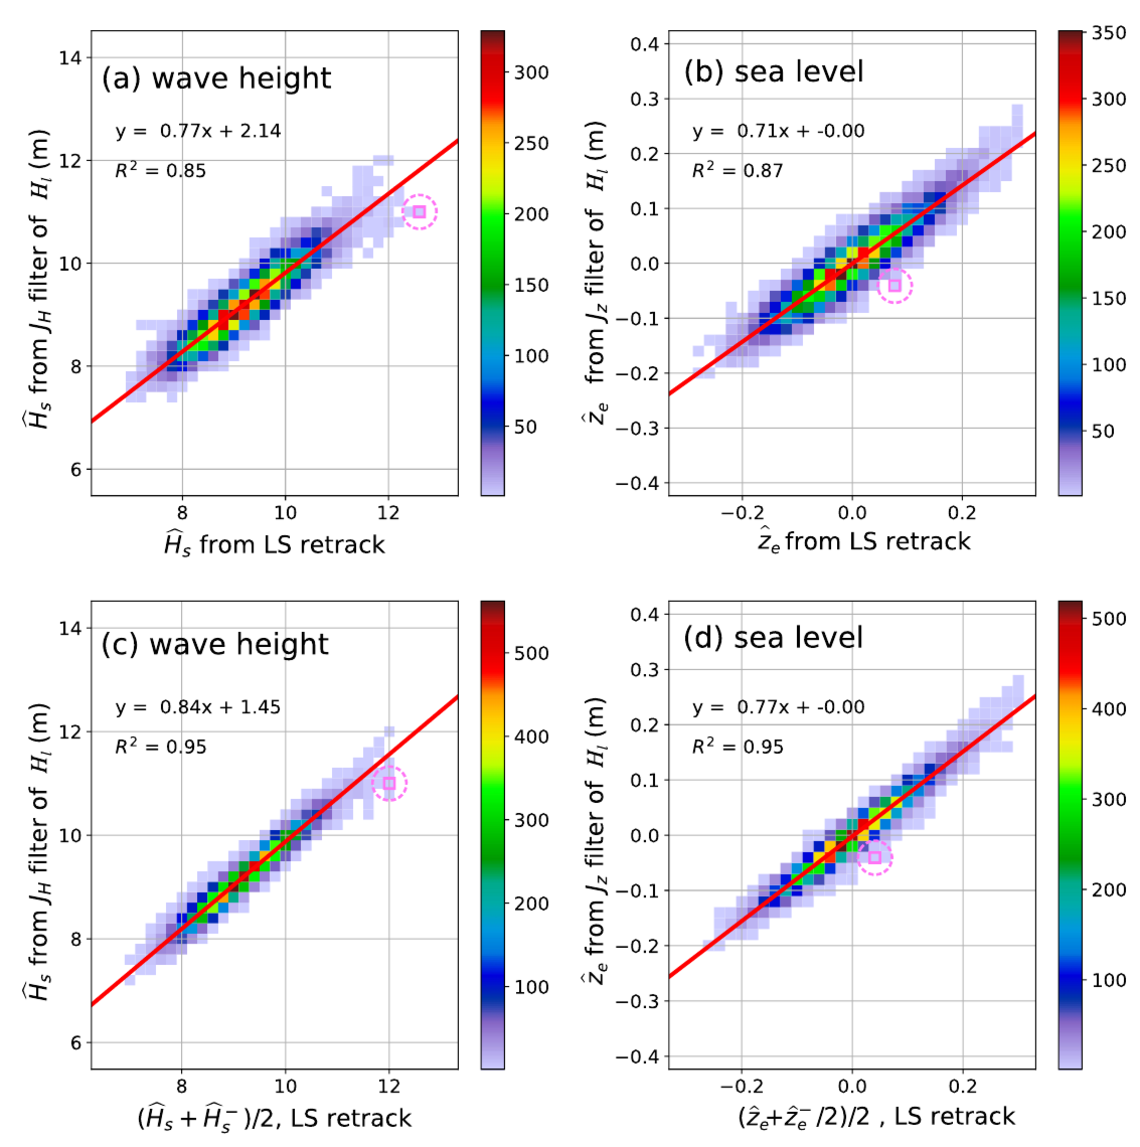
\includegraphics[width=0.7\textwidth]{FIGS_CH_SAT/verification-of-the-altimeter-doughnut-footprint-theory.png}}
%\vspace{3.64in}
  \caption{Verification of the doughnut theory: the retracked (a) wave height and (b) sea level is compared to the estimates using eqs. (\ref{eq:Hsfit}--(\ref{eq:epochfit}). In (c) and (d) the retracked values are averaged between the true surface and its mirror image (changing the sign of the elevation). This demonstrates that most of the residual not explained by the doughny theory is caused by the wave phases. The pixel highlighted with the dotted pink circle corresponds to Figure \ref{fig:alti_doughnut}.}{} \label{fig:alti_doughnut2}
\end{figure}
%%%%%%%%%%%%% end of figure 

This  analysis of the perturbation induced by wave groups can be adapted for speckle noise which can be treated as a random noise producing a random perturbation of the retracked parameters.  Both results can ne combined to build an uncertainty model for the altimeter measurements, and estimate the uncertainty of along-track averages. This allows a processing of the satellite data that removes the effect of wave groups in the altimeter measurements so that a truly significant wave height can be estimated from the data (and not a strangely averaged "local wave height"). For example, \cite{DeCarlo&Ardhuin2024} have revised the previous largest-ever measured wave height during storm Quirin from $\widehat{H}_s=20.1$~m \citep{Hanafin&al.2012} to $H_s=18.5 \pm 0.3$~m.

We may also expand the analysis to consider non-Gaussian effects of the surface elevation perturbation. In particular we can see that introducing a skewness of the elevation is equivalent to the effect of wave groups located at nadir \citep{Hayne1980,DeCarlo&Ardhuin2024}.

\section{The quest for better methods for nadir altimeters}
Most of the work on estimating parameters from altimeter data has focused on reducing the effect of speckle noise \citep{Challenor&Srokosz1989}. For speckle-dominated noise, it can be shown that the optimal cost functions is a  maximum likelihood (ML), which is a bit like fitting the waveform with a log scale instead of a linear scale, as illustrated on Figure \ref{fig:alti_linlog}.
%%%%%%%%%%%%% figure
\begin{figure}[h!]
\centerline{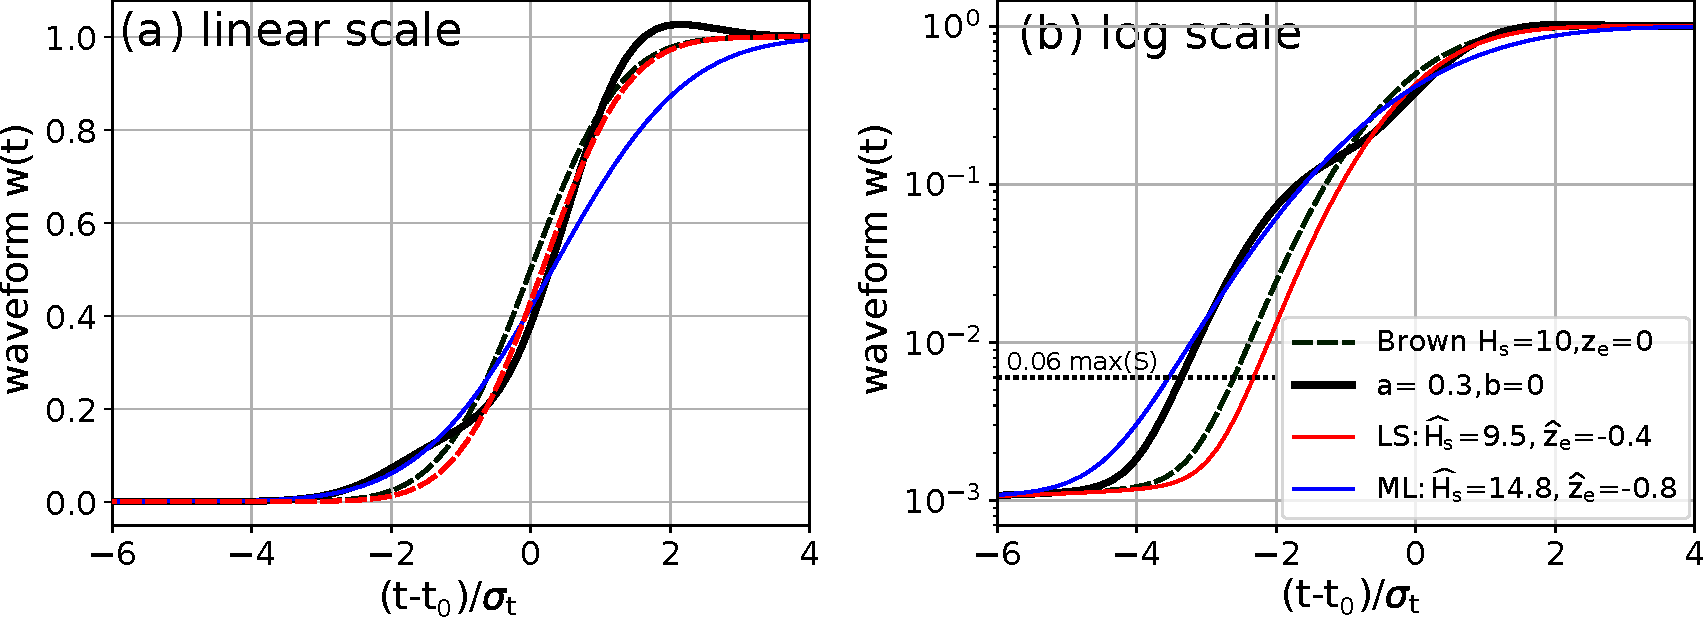
\includegraphics[width=\textwidth]{FIGS_CH_SAT/waveforms_lin_log.pdf}}
%\vspace{3.64in}
  \caption{Perturbed Brown waveform and best fits using a Least Square (LS) cost function or a Maximum Likelihood cost function.}{} \label{fig:alti_linlog}
\end{figure}
%%%%%%%%%%%%% end of figure 
Because it puts a much stronger emphasis on the early part of the waveform, the effective footprint of the ML retracker is smaller than the doughnut footprint of the LS retracker, and it has a very different shape and a maximum sensitivity at nadir.  In fact the ML retracker is not optimal for sea states with very large values of $Q_{\mathrm{kk}}$.

All this could sound like unnecessary technical details, bur figure \ref{fig:alti_SWIM_fit} shows an example where these things are important: the estimates sea level fluctuations of the order of 0.5 m are spurious effects of the wave groups on the retracking procedure. They average out over large scales but gthat still leaves some strong noise at scales under 100 km. 
%%%%%%%%%%%%% figure
\begin{figure}[h!]
\centerline{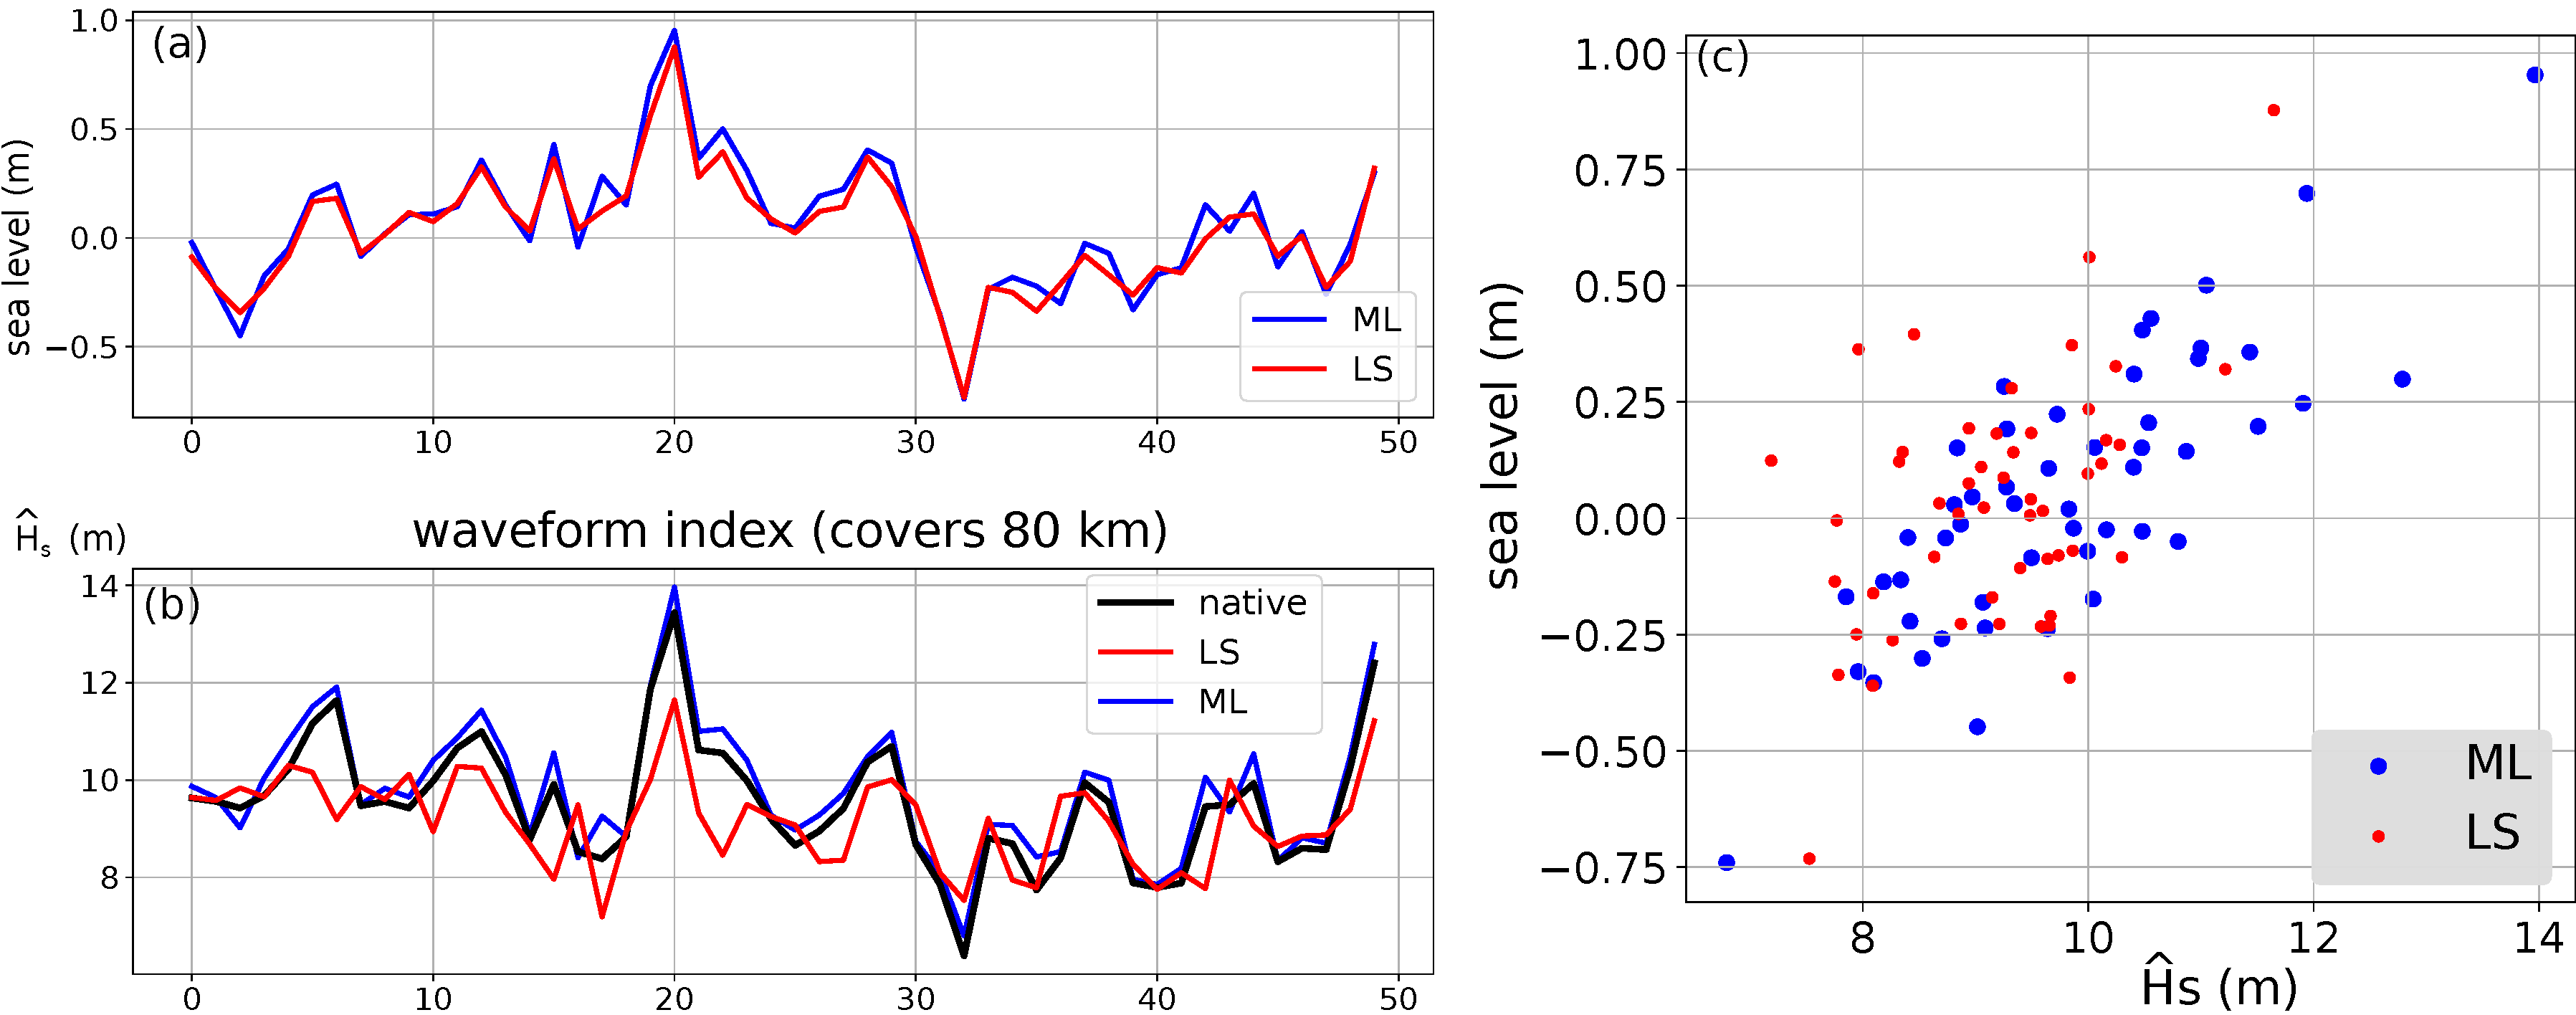
\includegraphics[width=\textwidth]{FIGS_CH_SAT/SWIM_data_LS_vs_ML.pdf}}
%\vspace{3.64in}
  \caption{Estimates of the (a) sea level $\widehat{z}_e$ and (b) wave heights $\widehat{H}_s$ for 50 consecutive waveforms of 
 CFOSAT corresponding to the spectrum in figure 5.5.b. This uses two different cost
functions: LS is a least squares fit and ML is a maximum likelihood fit to the same theoretical waveform. The native data is shown for reference and is the operational method as described in Tourain et al. (2021). The good agreement of the ML retracking
with the native data requires to ignore the first range gates using $k_{\min}\simeq 80$, 
or adapting kmin such that $w (k_{\min}) > r_{\min} \max (w)$,
 with $r_{\min} \simeq 0.06$. \label{fig:alti_SWIM_fit} }
\end{figure}
%%%%%%%%%%%%% end of figure 



Other interesting alternative exists: the $C_{LS}$ cost function can be modified to introduce weights. Taking weights inversely proportional to the theoretical Brown waveform is a good choice that is now further investigated. A complementary approach is to  filter the data using the series of measurements along the satellite track \citep{Quilfen&Chapron2019}.



It should be noted that the main application of the altimeters was the mapping of the sea surface height (SSH) for the determination of the geoid, tides and dynamical topography. The measured
 SSH can be much more precise than $dr$, thanks to averaging. Waves play an important role in the estimation of the SSH because of a range bias induced by wave non-linearities that induce a correlation between the local surface slope variance (and this its brightness for the radar) and the surface elevation \citep{Jackson1979,Srokosz1986}. This is known as 
 the sea state bias, and on average it is of the order of
 3~\% of Hs \citep[e.g.][]{Minster&al.1992}. 
 
 Also, because $H_s$ and SSH are estimated jointly using a parametric fit to the waveform, there are important correlated errors in the two parameters \citep[e.g.][]{Dibarboure&al.2014,DeCarlo&al.2023}. 
 %%%%%%%%%%%%% figure
\begin{figure}[htb]
\centerline{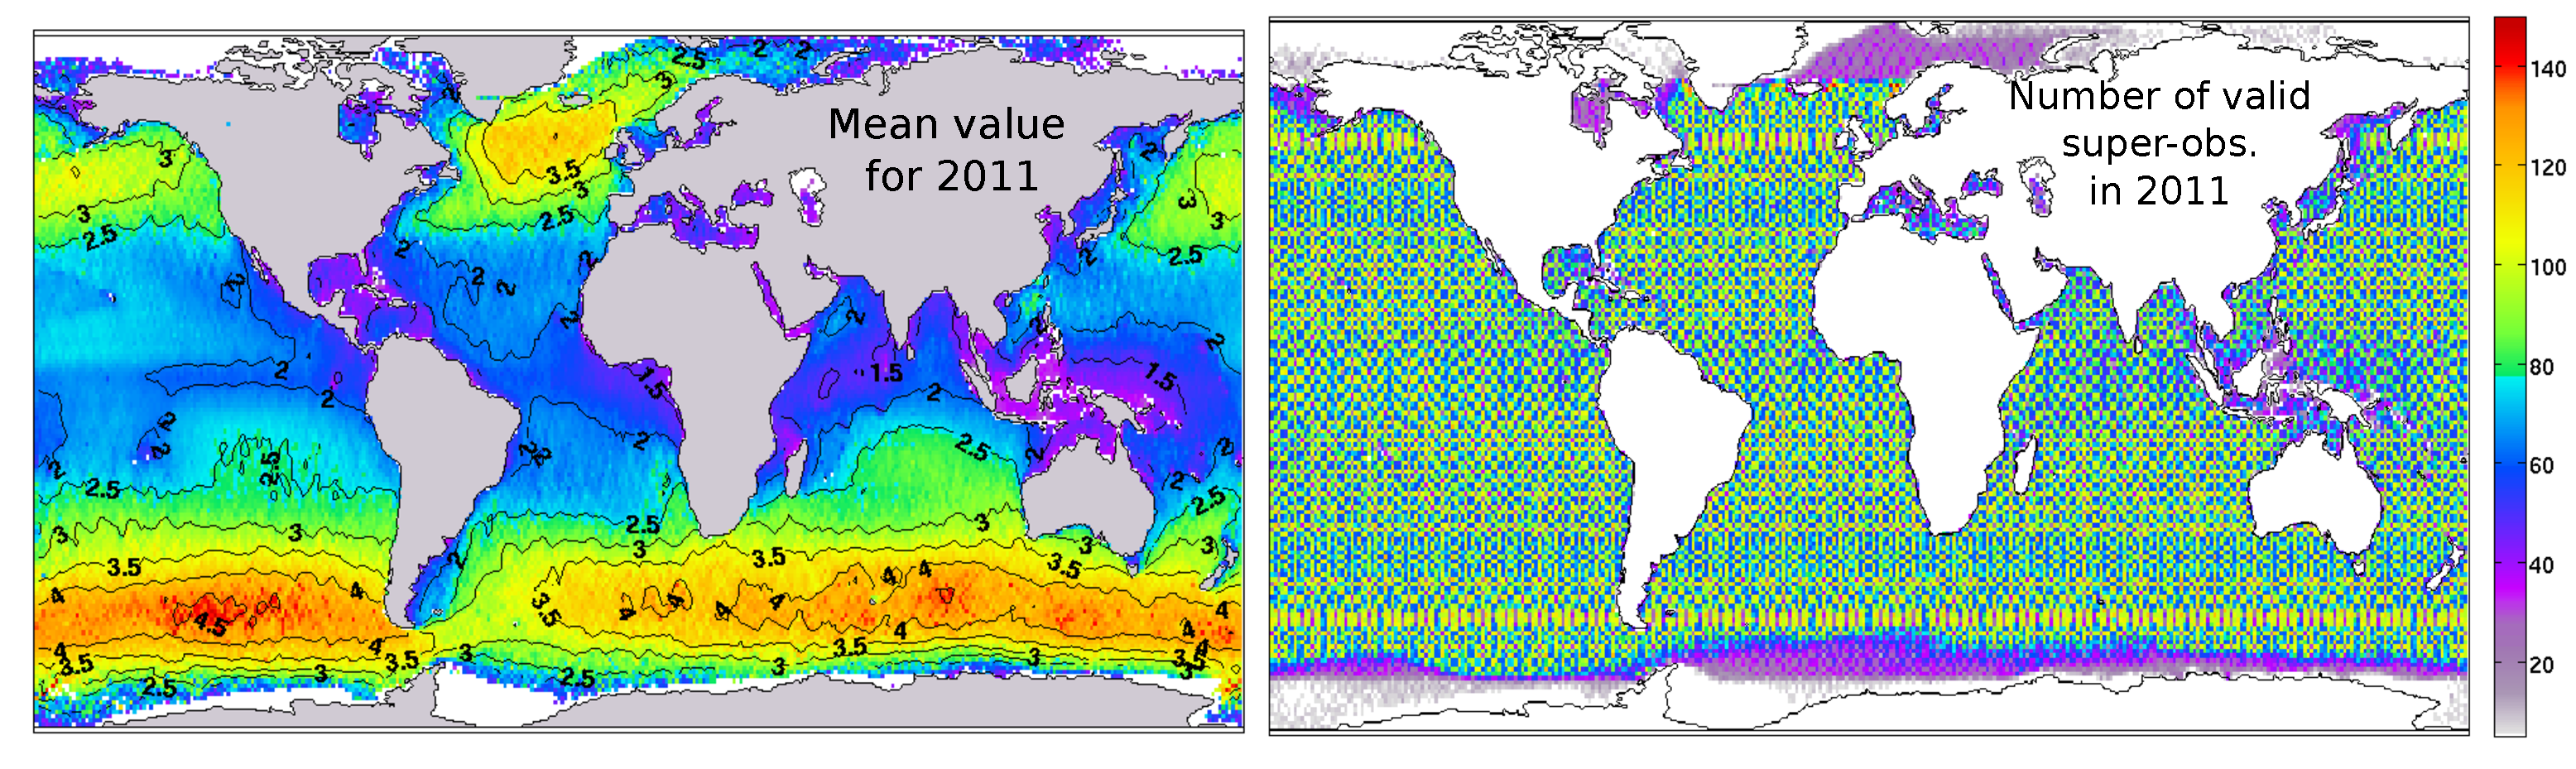
\includegraphics[width=\textwidth]{FIGS_CH_SAT/altimetre_cartes2011.pdf}}
%\vspace{3.64in}
  \caption{Global coverage of satellite altimeters}
    {Over one day, the 3 satellites Jason 2, Cryosat 2 and SARAL/AltiKa covered all the oceans and seas with a density high enough to capture all the 
important storms. In a year, the full ocean is covered at a resolution of 1 degree in latitude and longitude.  
 Data provided by ESA and CNES and processed by Ifremer. The spatial 
cover depends on the orbits shape. The number of tracks per 1 degree x 1 degree box (bottom panel) varies
from 20 to 160 over a year: the coverage is less frequent close to the pole because Jason 2 has a more oblique orbit that does not cover the 
latitudes beyond 66 degrees. Also, sea ice  produces echoes that differ from those of water and prevent the estimation of the wave height.} 
\label{fig:altimeter_coverage}
\end{figure}
%%%%%%%%%%%%% end of figure



\section{delay-Doppler altimetry}\label{section:delay-Doppler}
Another principle that can be used to refine the position and/or to measure the velocity of targets along the satellite flight path is the Doppler effect: fixed targets ahead of the radar are moving towards it, and hence have a higher frequency, while fixed targets that are behind along the satellite path 
are moving away, giving a lower radar frequency. Typical low Earth orbits give a satellite velocity around $V=7$~km/s. Hence, a Ka-band system at 36~GHz frequency will see a Doppler shift
of the order of $V f_r/c = 840$~kHz, which is further reduced by the incidence angle $\theta_r$. For a 0.5$^\circ$  antenna aperture, $\theta_r$ will 
normally vary between 0 and 0.5$^\circ$,  and the Doppler will be limited to 7.3~kHz.  

The main benefit of Delay-Doppler altimetry is the increase of the number of "independent looks" of the sea surface, which helps reduce Speckle noise, but cannot do anything about the true geophysical variability induced by wave groups. Delay-Doppler altimetry has also been developed to separate echoes along the track, which is particularly useful for measuring sea ice freeboard at the edges of sea ice leads, hence its first implementation on Cryosat-2. 


A slicing of the radar echoes according to their Doppler shift allows a high-resolution mapping of the surface along the satellite track. 
This principle is used on  Cryosat-2, Sentinel-3, and Sentinel-6 (Mike Freilich) with a standard processing giving 300~m resolution along the track, as shown on figure \ref{waveform}.d. In that case the basic 
data has now one extra dimension, making a `stack' of waveforms. For practical purposes, this stack is converted to a single `SAR mode' waveform, such as the solid lines 
shown in figure \ref{waveform}.b. 
At such a  resolution, the surface elevation due to  very long swells propagating along the track can be resolved. 
A natural limit to this along-track resolving power is the fact that the sea surface is moving up and down with the waves. Indeed, an orbital velocity 
of $w=2$~m/s gives a $u f_r / c=$ Doppler shift that can be mis-interpreted as a difference in incidence angle $\theta_r$ such that  
$(u f_r / c)=(V \sin\theta_r  f_r/c)$, this corresponds to a horizontal displacement $u H_r/V \simeq 200$~m for a radar altitude 
$H_r = 800$~km. 


%\subsubsection{Interferometric systems}



 \subsection{Synthetic Aperture Radars (SARs)}
As  explained above, the separation of echoes in the range direction is easily achieved by combining the delay and frequency modulation of 
the chirped radar signal, with a resolution in distance that is thus controled by the frequency bandwidth. 
In the other direction (azimuth), the simultaneous echoes can be separated by their Doppler shift. 
This is perfect if targets are fixed relative to the ground, and a 
very good resolution can be obtained, both in the range and azimuth directions (about 10~m for Envisat, 5~m for Sentinel 1 in wave mode and 1~m in spotlight mode for TerraSAR-X). This processing 
produces a  map of the surface 
backscatter in delay-Doppler coordinates. Unfortunately these positions are distorted from  true geographic positions when the surface is moving toward the 
radar. With a vertical velocity $w$, targets are displaced by $\delta=w \cos \theta_i  R/V$ along the azimuth direction. With a Sentinel-1 altitude $H_r = 693$~km  and a typical speed over ground $V=7.5$~km/s, when looking at an incidence angle of 23$^\circ$ the distance $R$ is close to\footnote{That approximation assumes a locally flat Earth. The exact value is obtained from the law of cosines in the triangle made of the satellite position, the target position and the center of the Earth, i.e. $R^2 + 2 R R_e \cos \theta_i +R_e^2 - (H_r +R_e)^2=0$, where $R_e$ is the radius of the Earth.} $H_r/\cos \theta_i$ and the 
factor $H_r/V$ is about 92~s$^{-1}$, i.e. a very small velocity  $w= 10$~cm/s gives a displacement in azimuth of $\delta=9.2$~m. 
A high speed train traveling at 100 m/s along tracks at $45^\circ$ with the range direction at an azimuth angle of 23$^\circ$ has a radial velocity of 28~m/s, would be displaced 2.7~km in the azimuth direction, at a location that is 2~km \textit{away} from the tracks!
%Figure \ref{fig:SAR_cars} shows an example of targets displaced from their true locations according to their azimutal speed. 
%
%
%%%%%%%%%%%%% figure
%\begin{figure}[htb]
%\centerline{\includegraphics[width=0.7\textwidth]{FIGURES/SAR_cars.pdf}}
%  \caption{Where is the fast car? it is in the optical picture, but out of the SAR `image'!}
%    {Images of cars with different velocities along an airport runway in a nominally processed radar image (left) and 
%a reference optical image (right), adapted from \cite{Palubinskas&al.2005}. The SAR acquisition was made from a Do-228 aircraft 
%flying at only 88 m/s and altitude 3.94~km, giving a ratio $H_r/V=44$~s$^{-1}$.} 
%\label{fig:SAR_cars}
%\end{figure}
%%%%%%%%%%%%%% end of figure


%%%%%%%%%%%%% figure
\begin{figure}[htb]
\centerline{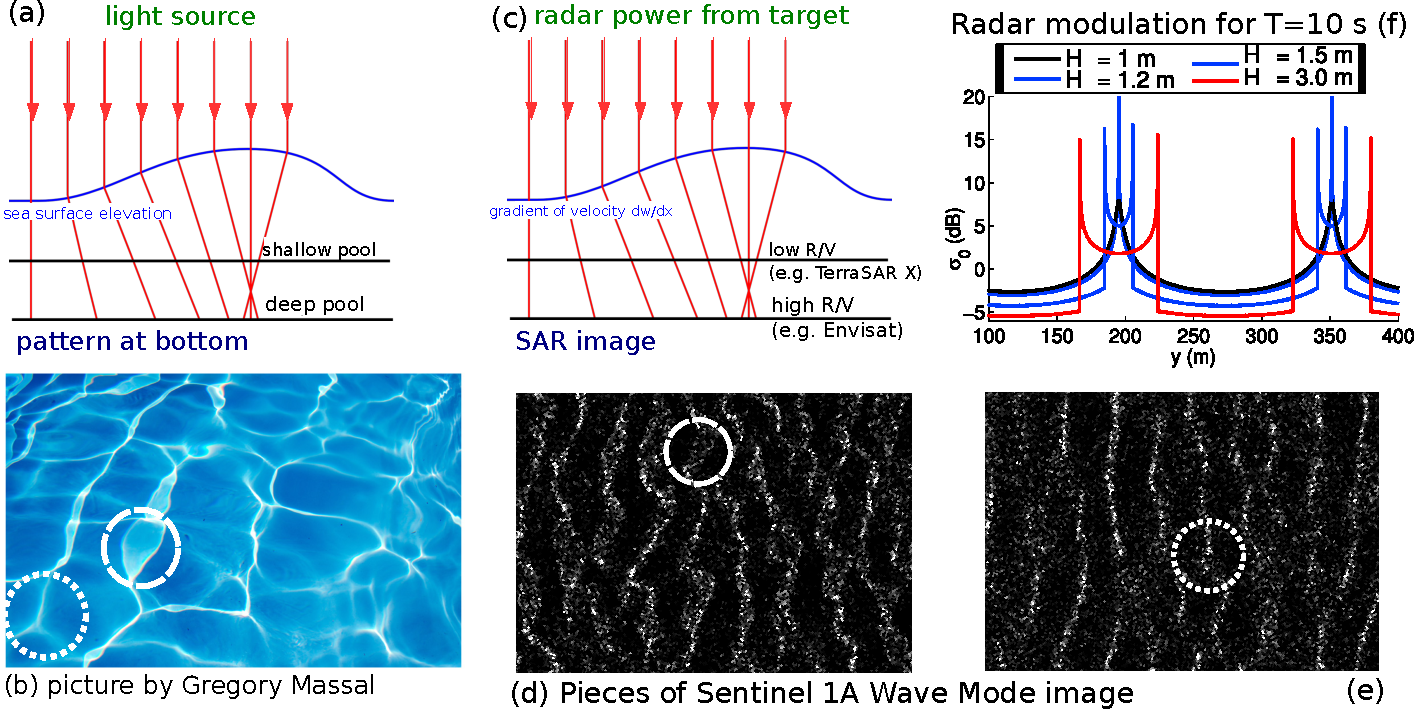
\includegraphics[width=0.8\textwidth]{FIGS_CH_SAT/dessin_fig1_landscape.pdf}}
%\vspace{3.64in}
  \caption{Patterns in SAR images}
    {Analogy between (a,b) light patterns at the bottom of a shallow pool, and (c,d,e) velocity bunching effects
in SAR images of ocean waves. (d) and (e) are taken from a wave mode Sentinel 1A image, acquired on 9 September 2014 at 04:48:16 UTC, 
at 10 and 35~km inside of the sea ice. In (d), almost all crests are doubled, for example in the region within the dashed circle. 
In (e) the lines are less bright and not doubled (for example within the dotted circle). This is easily simulated, as shown in (f), with the variations of image intensity
expected from a sinusoidal monochromatic wave of wavelength 156~m \citep[Adapted from ][]{Ardhuin&al.2017}.} 
\label{fig:SAR_pool}
\end{figure}
%%%%%%%%%%%%% end of figure
In the case of  waves motion a velocity bunching effect appears, the echoes on the image are shifted from their actual
position depending on the surface velocity towards the satellite creating a pattern of brighter areas, where the displaced targets are `bunched 
together', and darker regions. This mechanism is often the main cause of the wave-induced $\sigma_0$ modulation in the open ocean. 
In ice-covered water, this is probably the only mechanism present that creates wave patterns in SAR images. This bunching in the azimuth direction is very 
similar to the light patterns at the bottom of a shallow pool that are caused by light refraction, as illustrated in figure \ref{fig:SAR_pool}. 

%%%%%%%%%%%%%%%%%%%%%%%%%%%%%%%%%%%%%%%%%%%%%%%
%\begin{figure}[htb]
%\centering
%\includegraphics[width=\linewidth]{FIGURES/Nov1_for_book.pdf}
%\caption{Context of the  Sentinel-1A image acquired on November 1st, 2015, at 17:23 UTC, and available in situ data. The full image at 
%full resolution can be viewed at \href{http://bit.ly/22JFruo}{http://bit.ly/22JFruo}. (a) SAR-derived
%roughness (gray scale) showing open water between the Alaska shoreline, to the West of Barrow, and the measurement locations in the red box. 
%(b) Location of the R/V Sikuliaq and some of the measurement buoys. Note that buoy S15 is in open water. 
%(c) piece of the SAR image around the buoys S13 to W3. (d)  Directional spectrum estimated from S15 data using the Maximum Entropy Method.
%(e) Comparison of spectra derived from in situ data and the SAR image around buoy S13 and buoy W3. In each panel the spectrum at the offshore buoy S15 is 
%indicated for reference. The 'cut-off' effect is the reduction of wave spectrum according to eq. (\ref{eq:cutoff}). Adapted from \cite{Ardhuin&al.2017}.}
%\label{fig:nov1}
%\end{figure}
%%%%%%%%%%%%%%%%%%%%%%%%%%%%%%%%%%%%%%%%%%%%%%%
In the case of a monochromatic wave train propagating in the azimuth ($y$) direction, with wavenumber $k_y$, and not located right under the satellite but at an icidence angle $\theta_i$, 
the target displacement in the SAR image due to the velocity towards the satellite is 
\begin{equation}
 \delta = \left ( W \cos (k_y  y - \sigma t) \cos \theta_i  + U \sin (k_y  y - \sigma t) \sin  \theta_i  \right) H_r/(V \cos \theta). \label{eq:delA}
\end{equation}
where $U$ and $W$ are the amplitudes of the horizontal and vertical velocities given by eqs. (\ref{vitesse})-(\ref{eq:w}). 

Assuming a uniform radar power scattered from the sea surface $\sigma_0$, and taking the $y$ dimension  along the azimuth, 
the SAR image intensity is the incoherent sum at the displaced positions $y'$ of the power coming from the true pixel positions $y$, it is thus given by the inverse of Jacobian of the SAR displacements 
$y \rightarrow y'=y+\delta$, \citep[see eq. 21  in][]{Hasselmann&Hasselmann1991}, 
\begin{equation}
 J = \left|dy'/dy\right|,
\end{equation}
for a monochromatic wave of amplitude $a$ it is, 
\begin{equation}
I'_{SAR}(y) = \sigma_0/J = \sigma_0 / \left|1 -  C_{AR}  \sin( k_y y- \sigma t) \right|\label{ISAR}.
\end{equation}
The important parameter for image patterns is the coefficient $c$ in \cite{Alpers&Rufenach1979}, 
\begin{equation}
  C_{AR}=k_y (W + U \tan \theta_i) H_r/V.\label{eq:CAR_def}
\end{equation}


 For $C_{AR} << 1$, eq. (\ref{ISAR}) can be linearized, but as $C_{AR}$ increases, the SAR displacements become strongly nonlinear and for $C_{AR}= 1$, 
 the Jacobian is zero and $I'_{SAR}$ becomes infinite just like the light intensity at the focal point of a lens. 
In our figure 1.f, with a wave period of 10~s traveling in the azimuth direction, $C_{AR}= 1$  corresponds to an amplitude of the elevation $a=0.42$~m, 
which, for random waves of the same energy would be a significant wave height $H_s=4\sqrt(a^2/2)=1.2$~m. 
For $C_{AR} > 1$, each bright line becomes a doublet. The two lines of the doublet progressively drift apart as the amplitude increases, pulling 
the minimum intensity to lower and lower values, up to the point where lines 
from different doublets meet, at $ C_{AR} \simeq 4.6$. Beyond this value there is no region of very low intensity anymore. 
%For waves  in  sea ice, this can be inverted for  $C_{AR}$ less than about 2 to give a map of orbital velocities and from that the wave spectra \citep{Ardhuin&al.2016b}.

In practice, except far inside the  sea ice cover, there are also short wave components in the wave spectrum $E(\kb)$. From a SAR processing point of view, 
these short waves are equivalent to Gaussian random vertical oscillations 
of $<v^2>$ leading to random displacements in the SAR image that are larger than their wavelengths and that do not produce any pattern. These short 
waves also reduce the contrast of longer components. \cite{Hasselmann&Hasselmann1991} gave a theoretical derivation of the impact of random waves on a SAR image spectrum $E_S(\kb)$,
their eq. (55), with a simplified derivation by \cite{Krogstad1992}. In practice the short wave effect is a reduction in the image spectrum by an exponential factor,  
\begin{eqnarray}
 E_S(\kb)&\simeq& \exp(-k_y^2 <v^2> H_r^2/V^2) E_l (\kb) = \exp(-k_y^2 \lambda_c^2/(2 \pi)^2 ) |M_S|^2 \left(E(\kb)+E(-\kb)\right)/2 , \label{eq:cutoff}
\end{eqnarray}
in which $E_l(\kb)$ is a linearized spectrum, based on a modulation transfer function $M_S$ that includes a linearized velocity bunching term, a hydrodynamic term due to the short scattering waves modified by 
longer waves, and a tilt term due to the change in local slope along long waves \citep{Hasselmann&al.1985,Hasselmann&Hasselmann1991}. All terms depend on the incidence angle, 
and these last two terms depend on the polarization of radar waves, horizontal or vertical, and on wind speed and wave age. 
The image is 
completely blurred at the scale of the random displacements and the resolution of 1 or 5~m is useless.


The azimuthal cut-off wavelength is $\lambda_c =  2 \pi \sqrt{<v^2>} H_r/V$, in which $<v^2>$ is the orbital velocity variance.  This cut-off effect is so dominant that it can 
actually be used to measure the surface orbital velocity variance from SAR images \citep{Stopa&al.2016}. A minor difficulty is the separation of the part of the wave spectrum that 
produces patterns in the SAR image and the shorter part that only introduces blurring. Looking at many ERS SAR data, \cite{Kerbaol1997} concluded that, in the case 
of a wind sea, the velocity variance $<v^2>$  should be restricted to waves shorter than a factor $f_L$ times the peak wavelength, with $f_L \simeq 0.33$ for a mean short wave direction 
in the range direction and  $f_L \simeq 0.15$ in the azimuth direction.  

Combining all these effects with some empirically derived MTFs, it was possible to estimate the heights of swells within 25\% of buoy measurements using 
wave mode data from Envisat \citep{Collard&al.2009}. The full significant wave height, including the waves shorter than $\lambda_c$ that are not resolved in the 
SAR image, can also be estimated by combining all image parameters \citep{Li&al.2011}. 






Several aspects of SAR processing are the subject of active research, including the measurement of high winds or currents, and improvements in the estimates of wave 
parameters in particular in ice-covered regions. 

%Figure \ref{fig:nov1} shows an example of waves around the ice edge: in the water (buoy S15), the waves cannot be seen by the SAR 
%because, with a peak wavelength of 100~m, they are much shorter than the 290~m cut-off wavelength. Waves only appear in the ice with an %increasing SAR spectral 
%density which is not due to an increase in wave height, but a reduction in the cutoff wavelength from $\lambda_c = 114$~m at S13 to  $\lambda_c = 87$~m at W3. Hence a correct estimation 
%of $\lambda_c$ is critical for a proper estimation of wave heights either in the open ocean or in ice-covered water. Another important practical problem, especially in ice-covered 
%region, is the presence of non-wave features in the image: boats, slicks, variations in wind speed, leads in ice... these usually show up in the low frequency part of the spectrum, 
%and, in figure \ref{fig:nov1} they probably are the reason for the spurious bump at $f=0.1$~Hz. 
 
Since SAR images are characterized by high resolution (5~m in the Sentinel-1 wave mode, 10~m in Interferometric Wide swath mode), and large coverage, they provide a unique opportunity 
to measure the spatial patterns in the wave field, as shown on figure \ref{SAR_exemple}.

%%%%%%%%%%%%% figure
\begin{figure}[!h]
\centerline{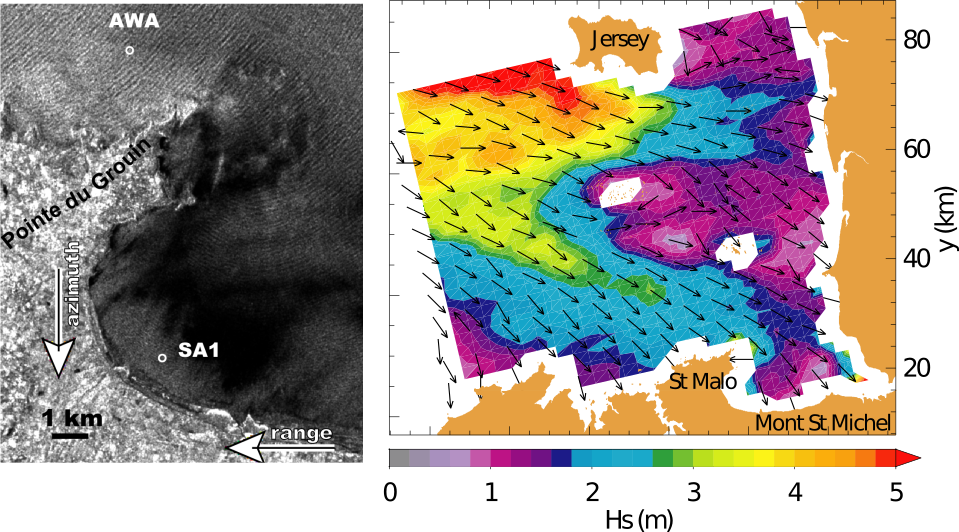
\includegraphics[width=0.8\textwidth]{FIGS_CH_SAT/Image_SAR_Cancale2.png}}
\caption{Left: Sample of a SAR image, recorded by Envisat  on March 9 2003, over French coast. The grey level is a function of the radar cross section that is modulated by waves. 
Right: Full image processed into wave spectra, with significant wave height and peak direction. AWA et SA1 are positions of in-situ instruments, 
used for validation \citep{Collard&al.2005}.}
\label{SAR_exemple}
\end{figure}
%%%%%%%%%%%%% end of figure



\subsection{SAR Across-track Interferometry: SWOT}
Compared to the SAR systems on Envisat and Sentinel-1 described above, the KaRIN instrument on SWOT has two very different features: first it measures at incidences very close to the vertical (nadir), and second it actually has 2 SAR systems forming a cross-track interferometric baseline. This means that in addition to the usual SAR imagery (a little unusual with KaRIN due to their incidence angles) we also get interferograms from the two SAR receivers on KaRIN, which provide a wealth of information: 
\begin{itemize}
\item the mean phase of the interferogram is related to the distance between the radar and the reflecting target, hence the sea surface elevation, which contains the geoid, the dynamic height, tides, internal waves... but also those wind-generated waves that are longer than the SAR pixel, as shown on Fig. \ref{fig:SWOTswell}. 
\item the noise of the interferometric phase is related to the distribution of these distances within a resolution pixel, hence the significant wave height of the waves that are not resolved by the surface height image. 
\end{itemize}

When trying to analyse SWOT data at small scales, it is thus really important to understand what is resolved, what is not, and how the unresolved surface elevations give spurious signals in the resolved part: indeed the imaging of the surface at near-nadir angles meas that all targets that have the same range will fall in the same pixel, even though they are not at the same $(x,y)$ position. This leads to a fairly nonlinear image-blurring or image-enhancing effect called "range-bunching": just like velocity bunching, which distorts or enhances the image in the azimuth direction, range bunching leads to distortions and blurring in range. You may look at the work by \cite{Peral&al.2015} before a more detailed summary appears in a new chapter. 

Figure \ref{fig:SWOTswell} and the cover of this book shows some example of wave signatures in SWOT surface elevation maps. A quantitative analysis was done by \cite{Ardhuin&al.2024} and revealed that SWOT is capable of measuring significan wave heights as low as 3~cm for wavelengths larger than 800~m: no other instrument can do this in the open ocean.
%%%%%%%%%%%%% figure
\begin{figure}[htb]
\centerline{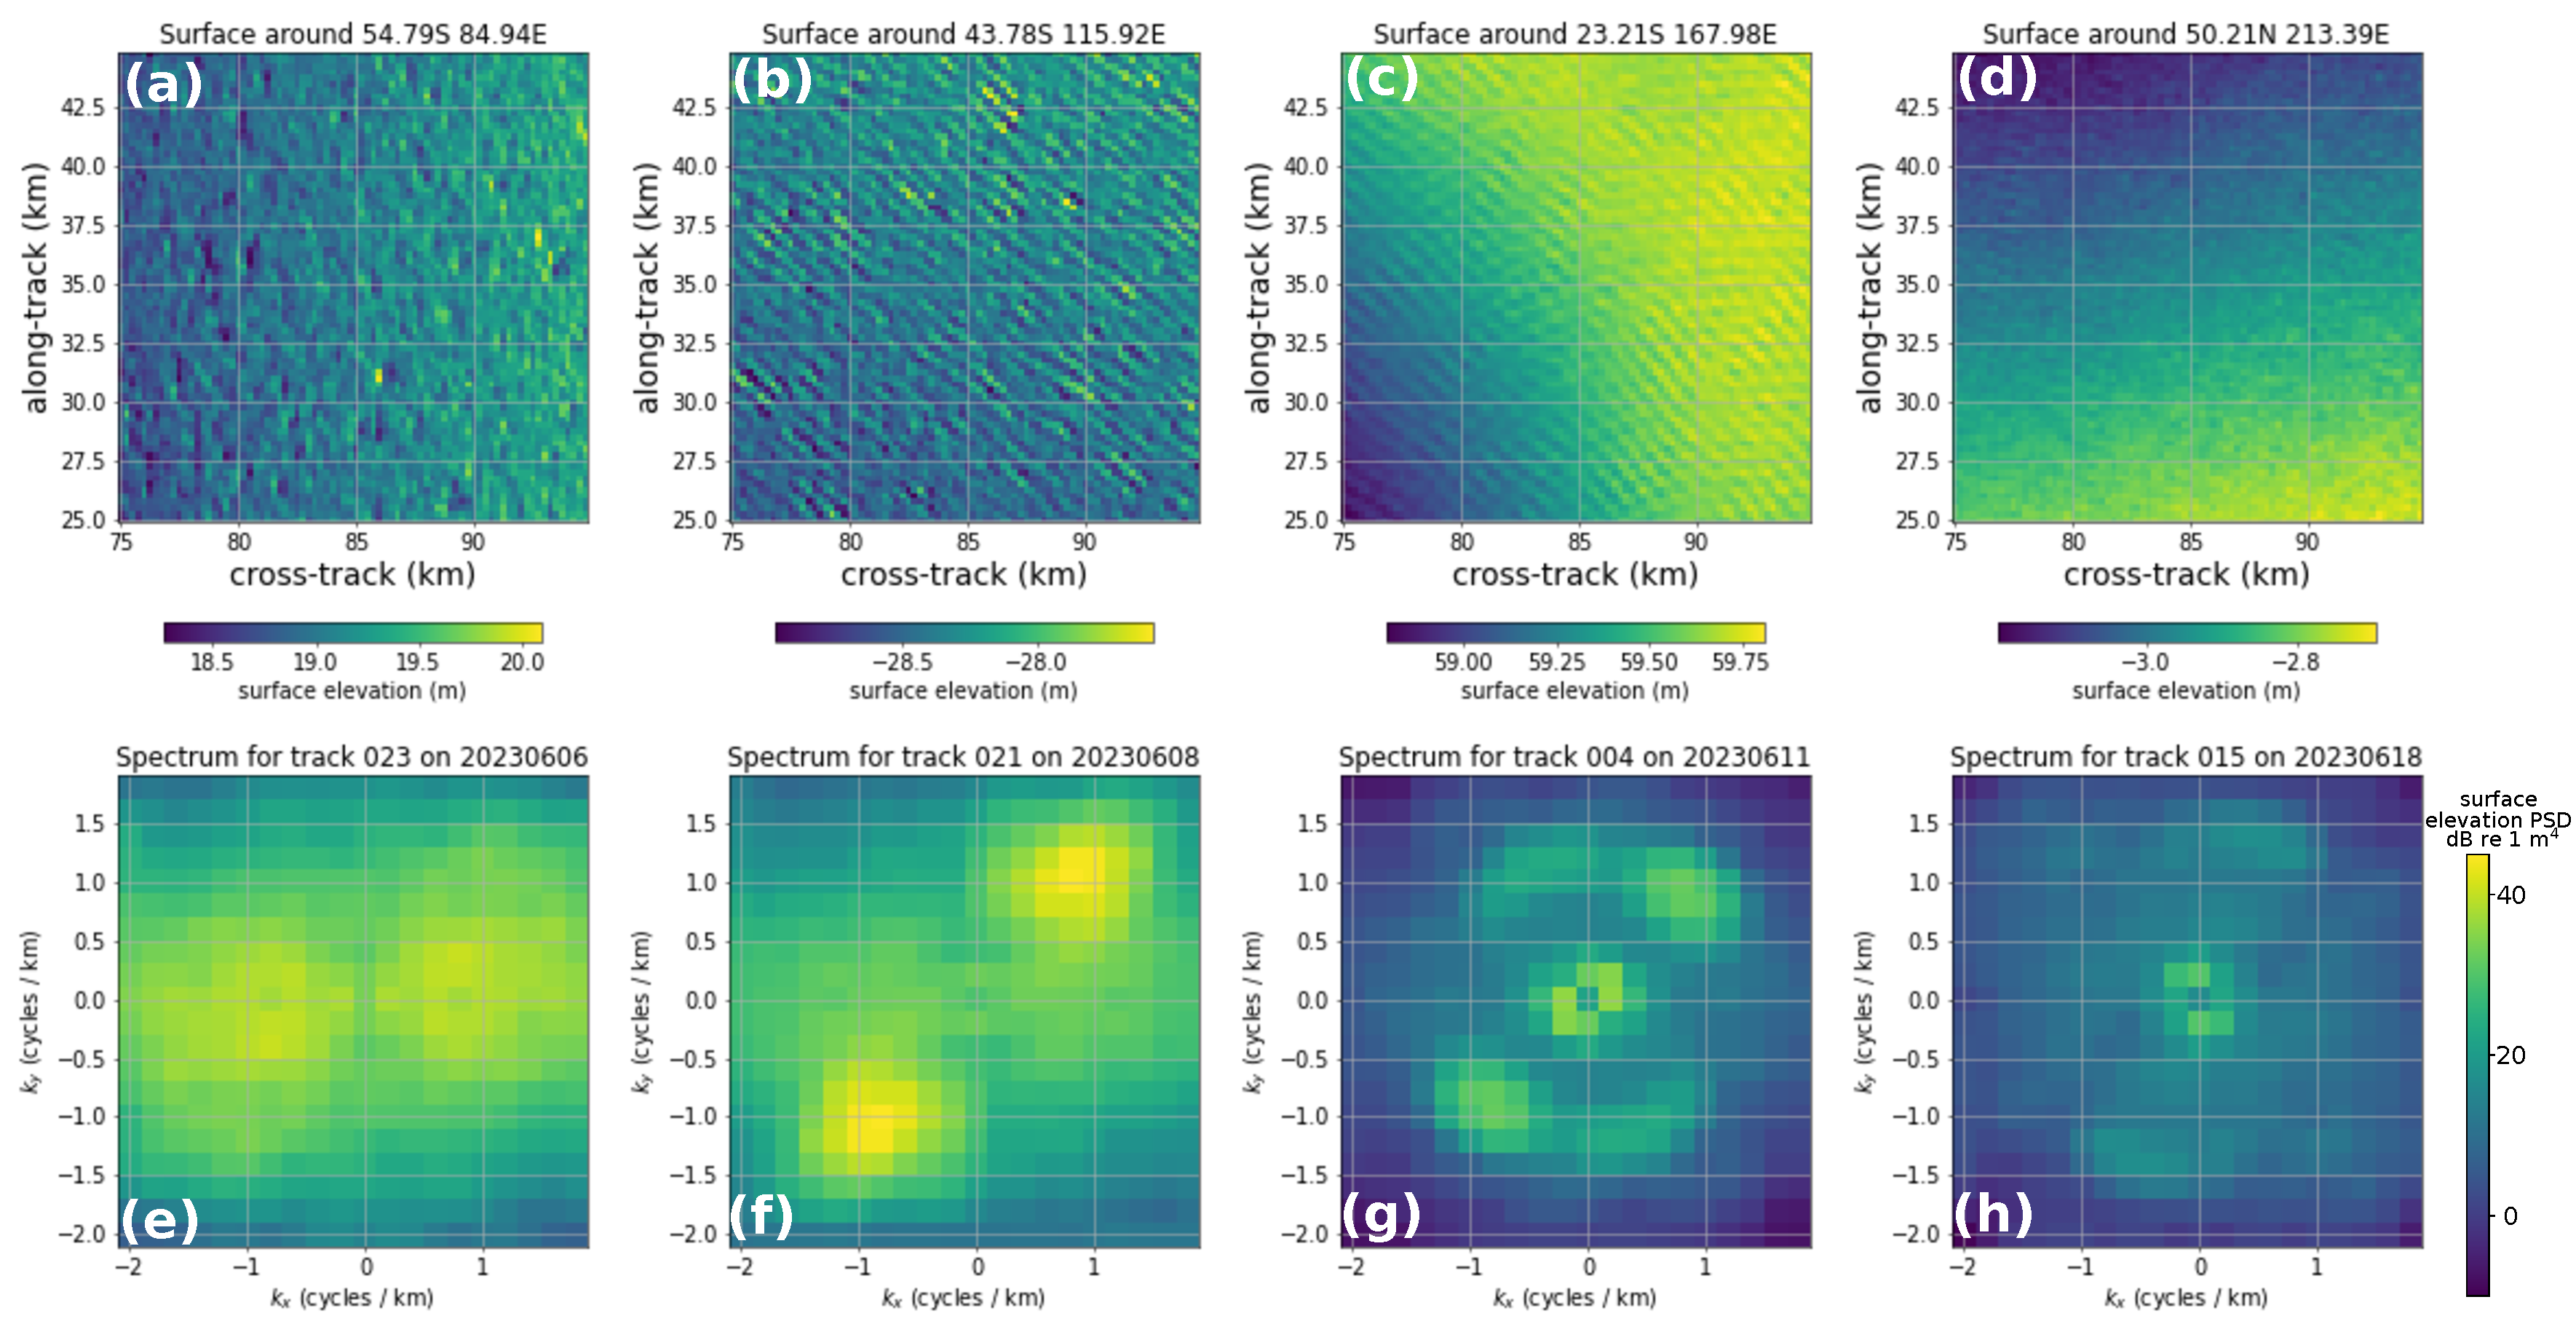
\includegraphics[width=\textwidth]{FIGS_CH_SAT/SWOTSWELL.pdf}}
\caption{Following swells with SWOT, from storm to the antipodes}{Top: small pieces (20 by 20 km) of SWOT data, bottom: corresponding surface elevation spectra $E(k_x,k_y)$, these are double-sided spectra. Left: in the storm on June 6 2023, south of Kergulen islands with strong range bunching effect. Next: large swells South of Australia, June 8. Next: refraction and diffraction over Antigonia seamount, south-east of New Caledonia, June 11. Right: small amplitude swells at ocean station Papa, Gulf of Alaska, on June 18, after 17,000~km of propagation.}
\label{fig:SWOTswell}
\end{figure}
%%%%%%%%%%%%% end of figure


\subsection{The wave spectrometer and the matching wavefront technique}
Whereas a SAR resolves the wave patterns in an image to produce a wave spectrum, 
it is possible to measure the 2D wave spectrum from a combination of 1D wave spectra. 
%%%%%%%%%%%%% figure
\begin{figure}[htb]
\centerline{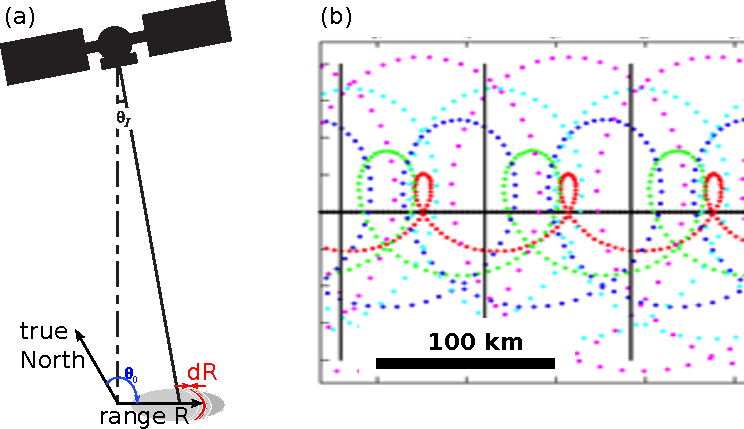
\includegraphics[width=0.4\textwidth]{FIGS_CH_SAT/CFOSAT_v2.pdf}}
\caption{Measurement principle  the SWIM radar that on CFOSAT. (a) geometry of the measurements for one cycle 
in direction $\theta_0$. The resolution in range $dR$ is of the order of 10~m, but the azimuth resolution is 18 km. Using different incidence angles $\theta_I$ (0, 2, 4, 6, 8 and 10 degrees) 
and rotating around the nadir provides estimates $E(k,\theta_0)$ in all direction $\theta_0$. (b) Coverage of the SWIM instrument on CFOSAT: each colored dot is the center 
of a 19~km diameter footprint.}
\label{CFOSAT}
\end{figure}
%%%%%%%%%%%%% end of figure

When echoes are combined from narrow strip in range (red band in figure 
\ref{CFOSAT}.a), the Fourier transform of these echoes in the range direction selects only the modulations by waves that are perfectly aligned with the direction 
$\theta_0$ to which the radar is looking, all other components cancel out.  Hence, the Fourier analysis of radar echoes provides a 1D spectrum  $E(k,\theta_0)$  
in the look direction. 
A successive acquisition in different directions provides the full directional spectrum $E(k,\theta)$.  
This is the principle of the wave spectrometer and it has been demonstrated with the airborne instrument
RAWS, developed by NASA \citep{Jackson&al.1985}, STORM and KuROS developed jointly by CNES and CNRS \citep{Hauser&al.1992,Caudal&al.2014}.
The first satellite wave spectrometer is SWIM, and it flies on the China-France Ocean Satellite (CFOSAT, Figure \ref{CFOSAT}), which was launched on October 29, 2018 \citep{Hauser&al.2021}. SWIM is unique in providing wave spectra co-located with classical altimeter measurements, allowing a much better understanding of historical altimeter data and their along-track variability \citep{DeCarlo&al.2023}, as detailed in chapter \ref{ch_groups}. 

%For larger incidence angles, the measurements cover a larger area of the ocean, but there is more sensitivity to the wind speed in the radar back-scatter. Hence, the SWIM  design is limited to 10 degrees of incidence. A larger incidence also requires a more powerful radar, because the reflectivity decreases with incidence angle. 

It is also possible to analyze the Doppler of the backscattered signal, as demonstrated with KuROS \citep{Caudal&al.2014}, but this is best done with a narrower antenna pattern as used from space. This additional measurement allows to remove the 180 degree ambiguity on the 
wave propagation direction, but it also provides an indepedant measuremnt of the wave spectrum via the orbital velocities, and finally it contains the signature of 
surface currents.  This Doppler capability to measure currents was included in the SKIM concept \citep{Ardhuin&al.2019e} and demonstrated with airborne measurements \citep{Marie&al.2020}.


